\chapter{Danh mục sơ đồ UML}
\label{app:uml}

Mã PlantUML của các sơ đồ nằm trong thư mục \code{docs/diagrams/}. Lệnh \code{scripts/docs/render-diagrams.sh} tải PlantUML (có kiểm tra mã băm SHA-1), render toàn bộ sơ đồ sang SVG trong \code{docs/diagrams/rendered/}, và dừng với mã lỗi khác 0 ngay ở sơ đồ đầu tiên sai cú pháp. Danh mục kèm liên kết nằm ở \code{docs/diagrams/INDEX.md}. Các hình trong thân khoá luận được vẽ lại với nhãn tiếng Việt và bố cục dọc cho vừa khổ A4; mã nguồn của chúng nằm trong \code{docs/khoa-luan-latex/hinh/puml/}.

\begin{table}{Danh mục 39 sơ đồ UML của nền tảng}
\label{tab:ds-uml}
\small
\begin{tabularx}{\textwidth}{|P{2.6cm}|r|L|}
\hline
\textbf{Góc nhìn} & \textbf{Số sơ đồ} & \textbf{Sơ đồ} \\ \hline
Use case & 4 & Toàn hệ thống; quản trị viên; thành viên hội đồng; tác tử \\ \hline
Lớp & 13 & Tổng quan mô hình miền; aggregate Agent, Project, Workflow; Strategy, Observer, Repository, Factory; vòng học; cộng tác tác tử; bộ máy quy trình; bảo mật, kiểm toán, tích hợp, báo cáo; phân tích, dự báo, chất lượng mã \\ \hline
Tuần tự & 11 & SD-001 tạo dự án; SD-002 chu trình suy nghĩ, hành động; SD-003 phê duyệt; SD-004 chuỗi giao việc; SD-005 học; SD-006 ảnh chụp và khôi phục; SD-007 lập trình cặp; SD-008 quy trình con; SD-009 gọi API bằng khoá API; SD-010 gửi webhook; SD-011 xuất dự án \\ \hline
Hoạt động & 4 & AD-001 vòng đời dự án; AD-002 quy trình có nhánh song song; AD-003 ước lượng công sức và chi phí; AD-004 phân tích và sửa chất lượng mã \\ \hline
Máy trạng thái & 4 & SM-001 tác tử; SM-002 lượt chạy quy trình; SM-003 công việc; SM-004 phê duyệt \\ \hline
Kiến trúc & 3 & Gói; thành phần; triển khai \\ \hline
\textbf{Tổng} & \textbf{39} & \\ \hline
\end{tabularx}
\end{table}

Một số sơ đồ gốc được in lại dưới đây để người đọc đối chiếu với mã nguồn.

\begin{figure}{Sơ đồ tuần tự SD-007: lập trình cặp có vòng làm rõ}
\label{fig:sd007}
\centering
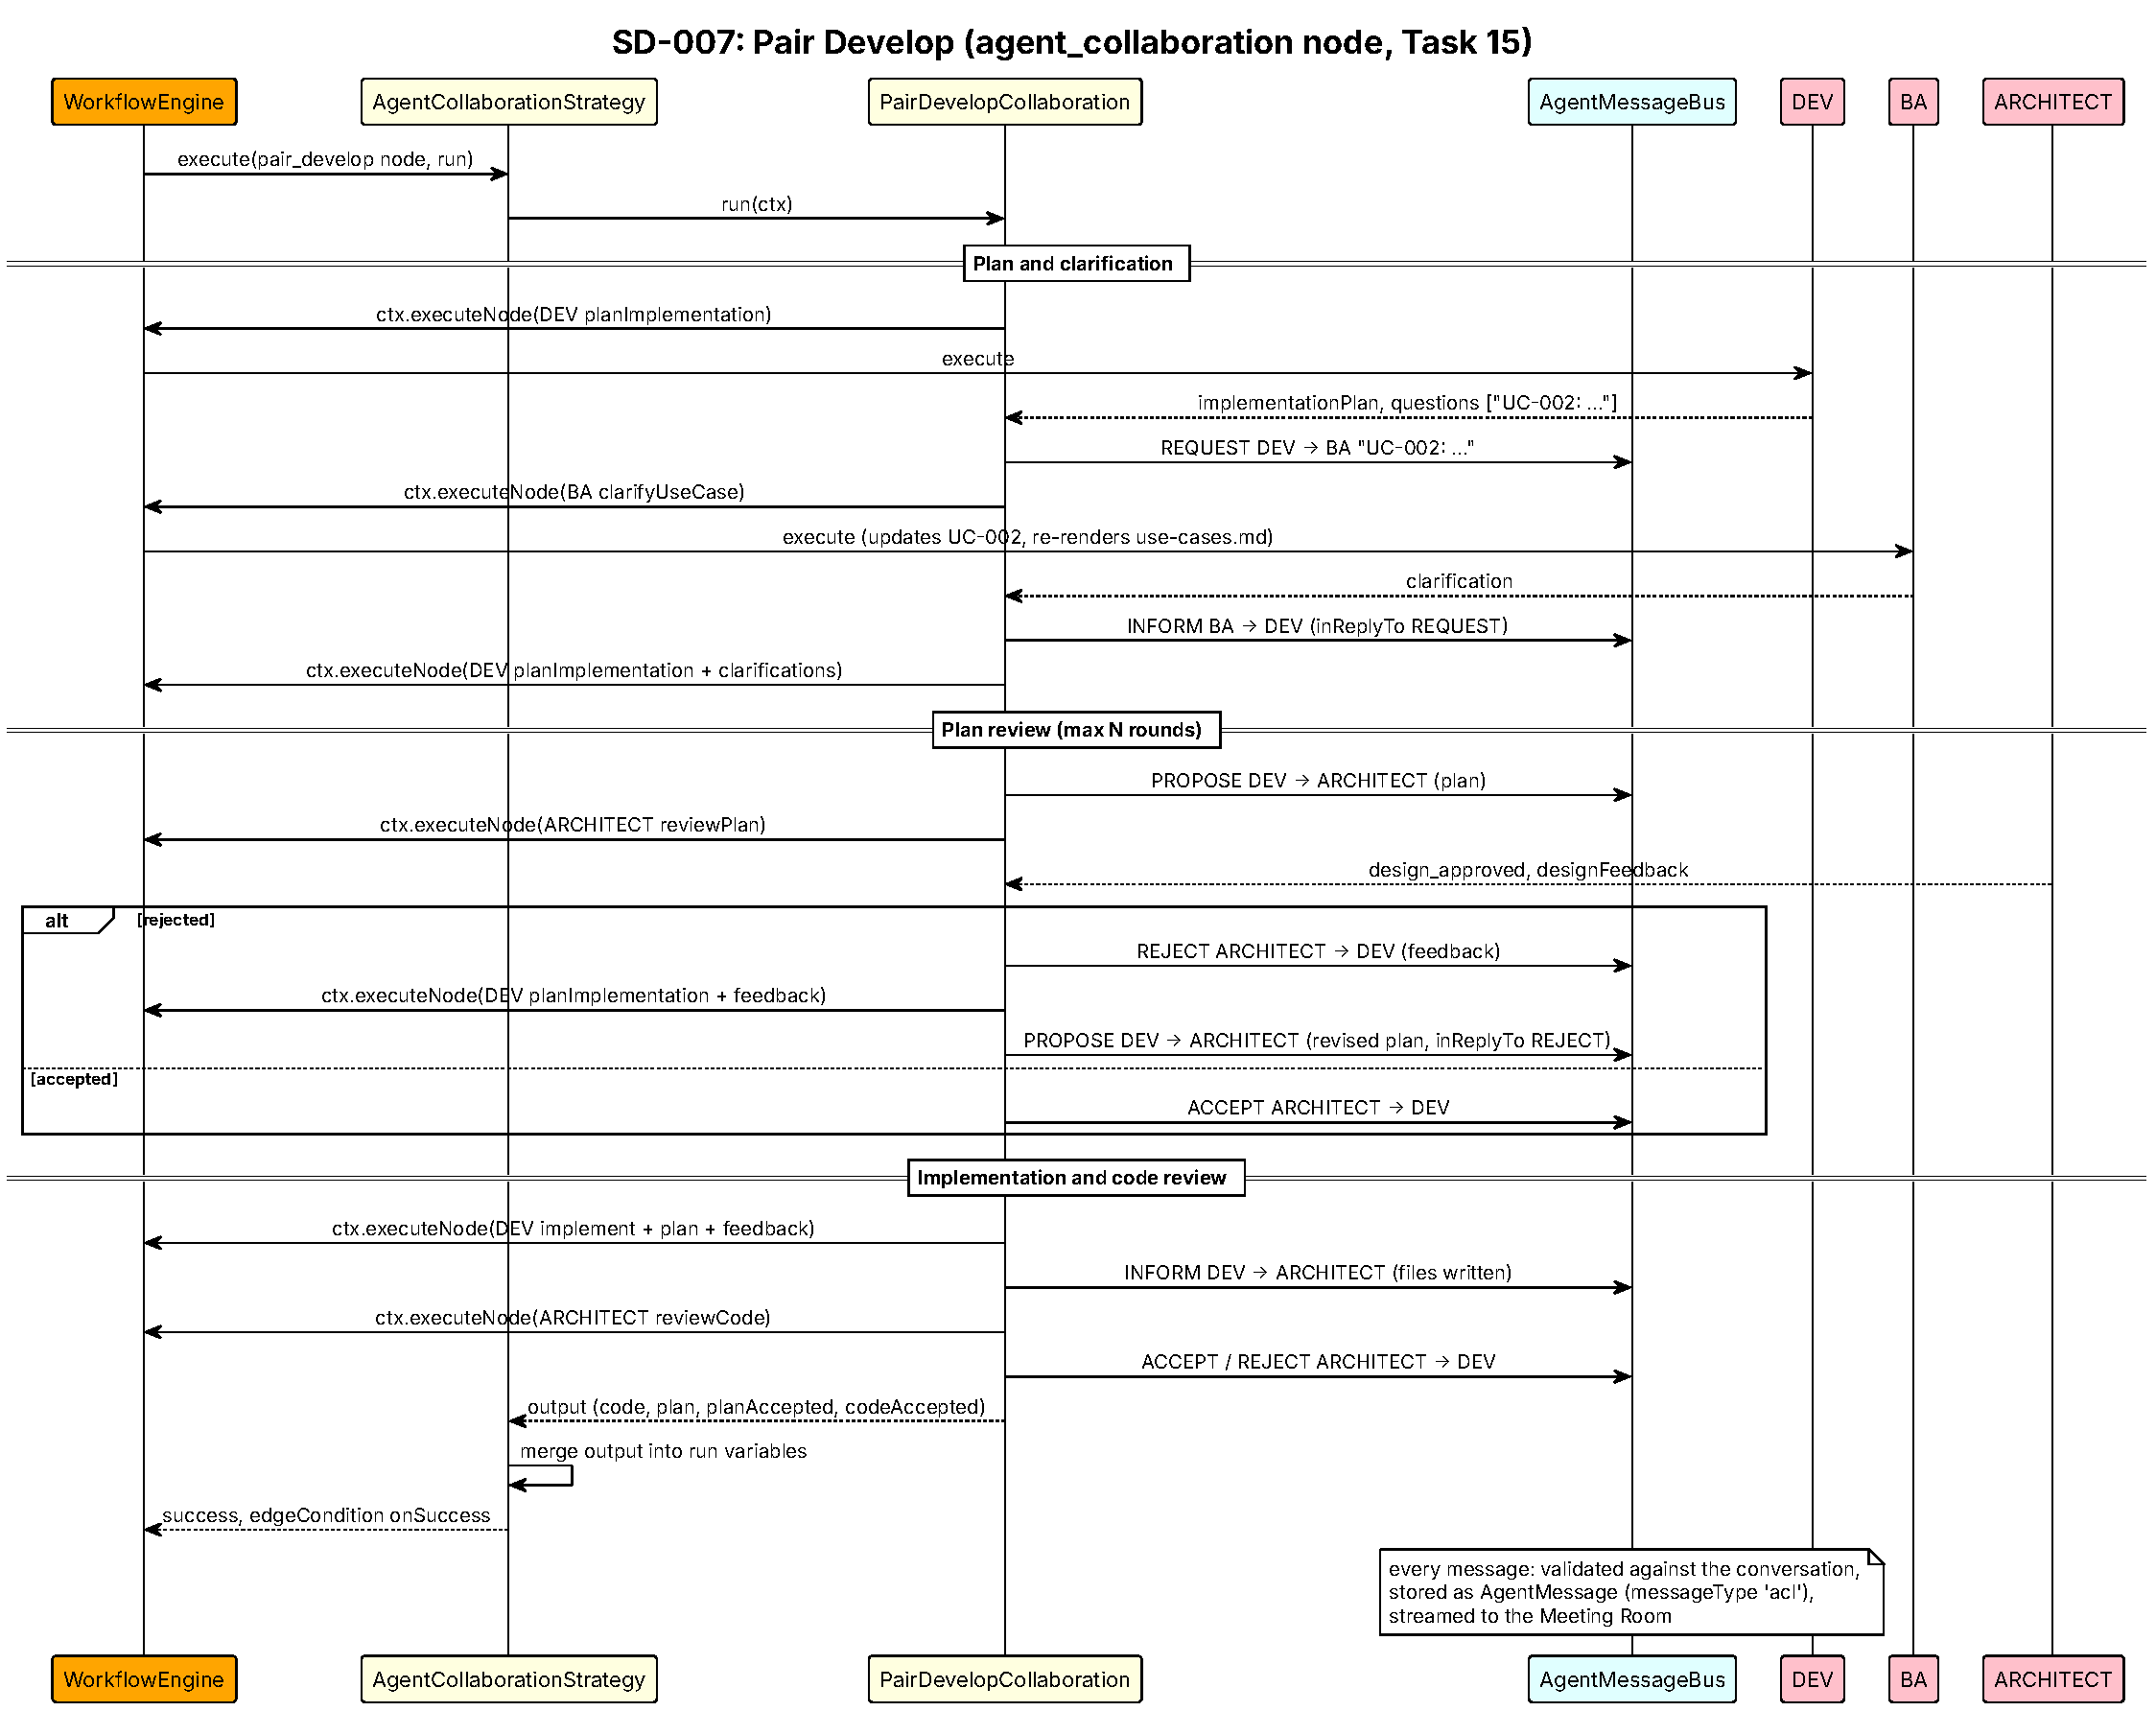
\includegraphics[width=\textwidth]{uml/SD-007-pair-develop.pdf}
\end{figure}

\begin{figure}{Sơ đồ tuần tự SD-008: thực thi quy trình con}
\label{fig:sd008}
\centering
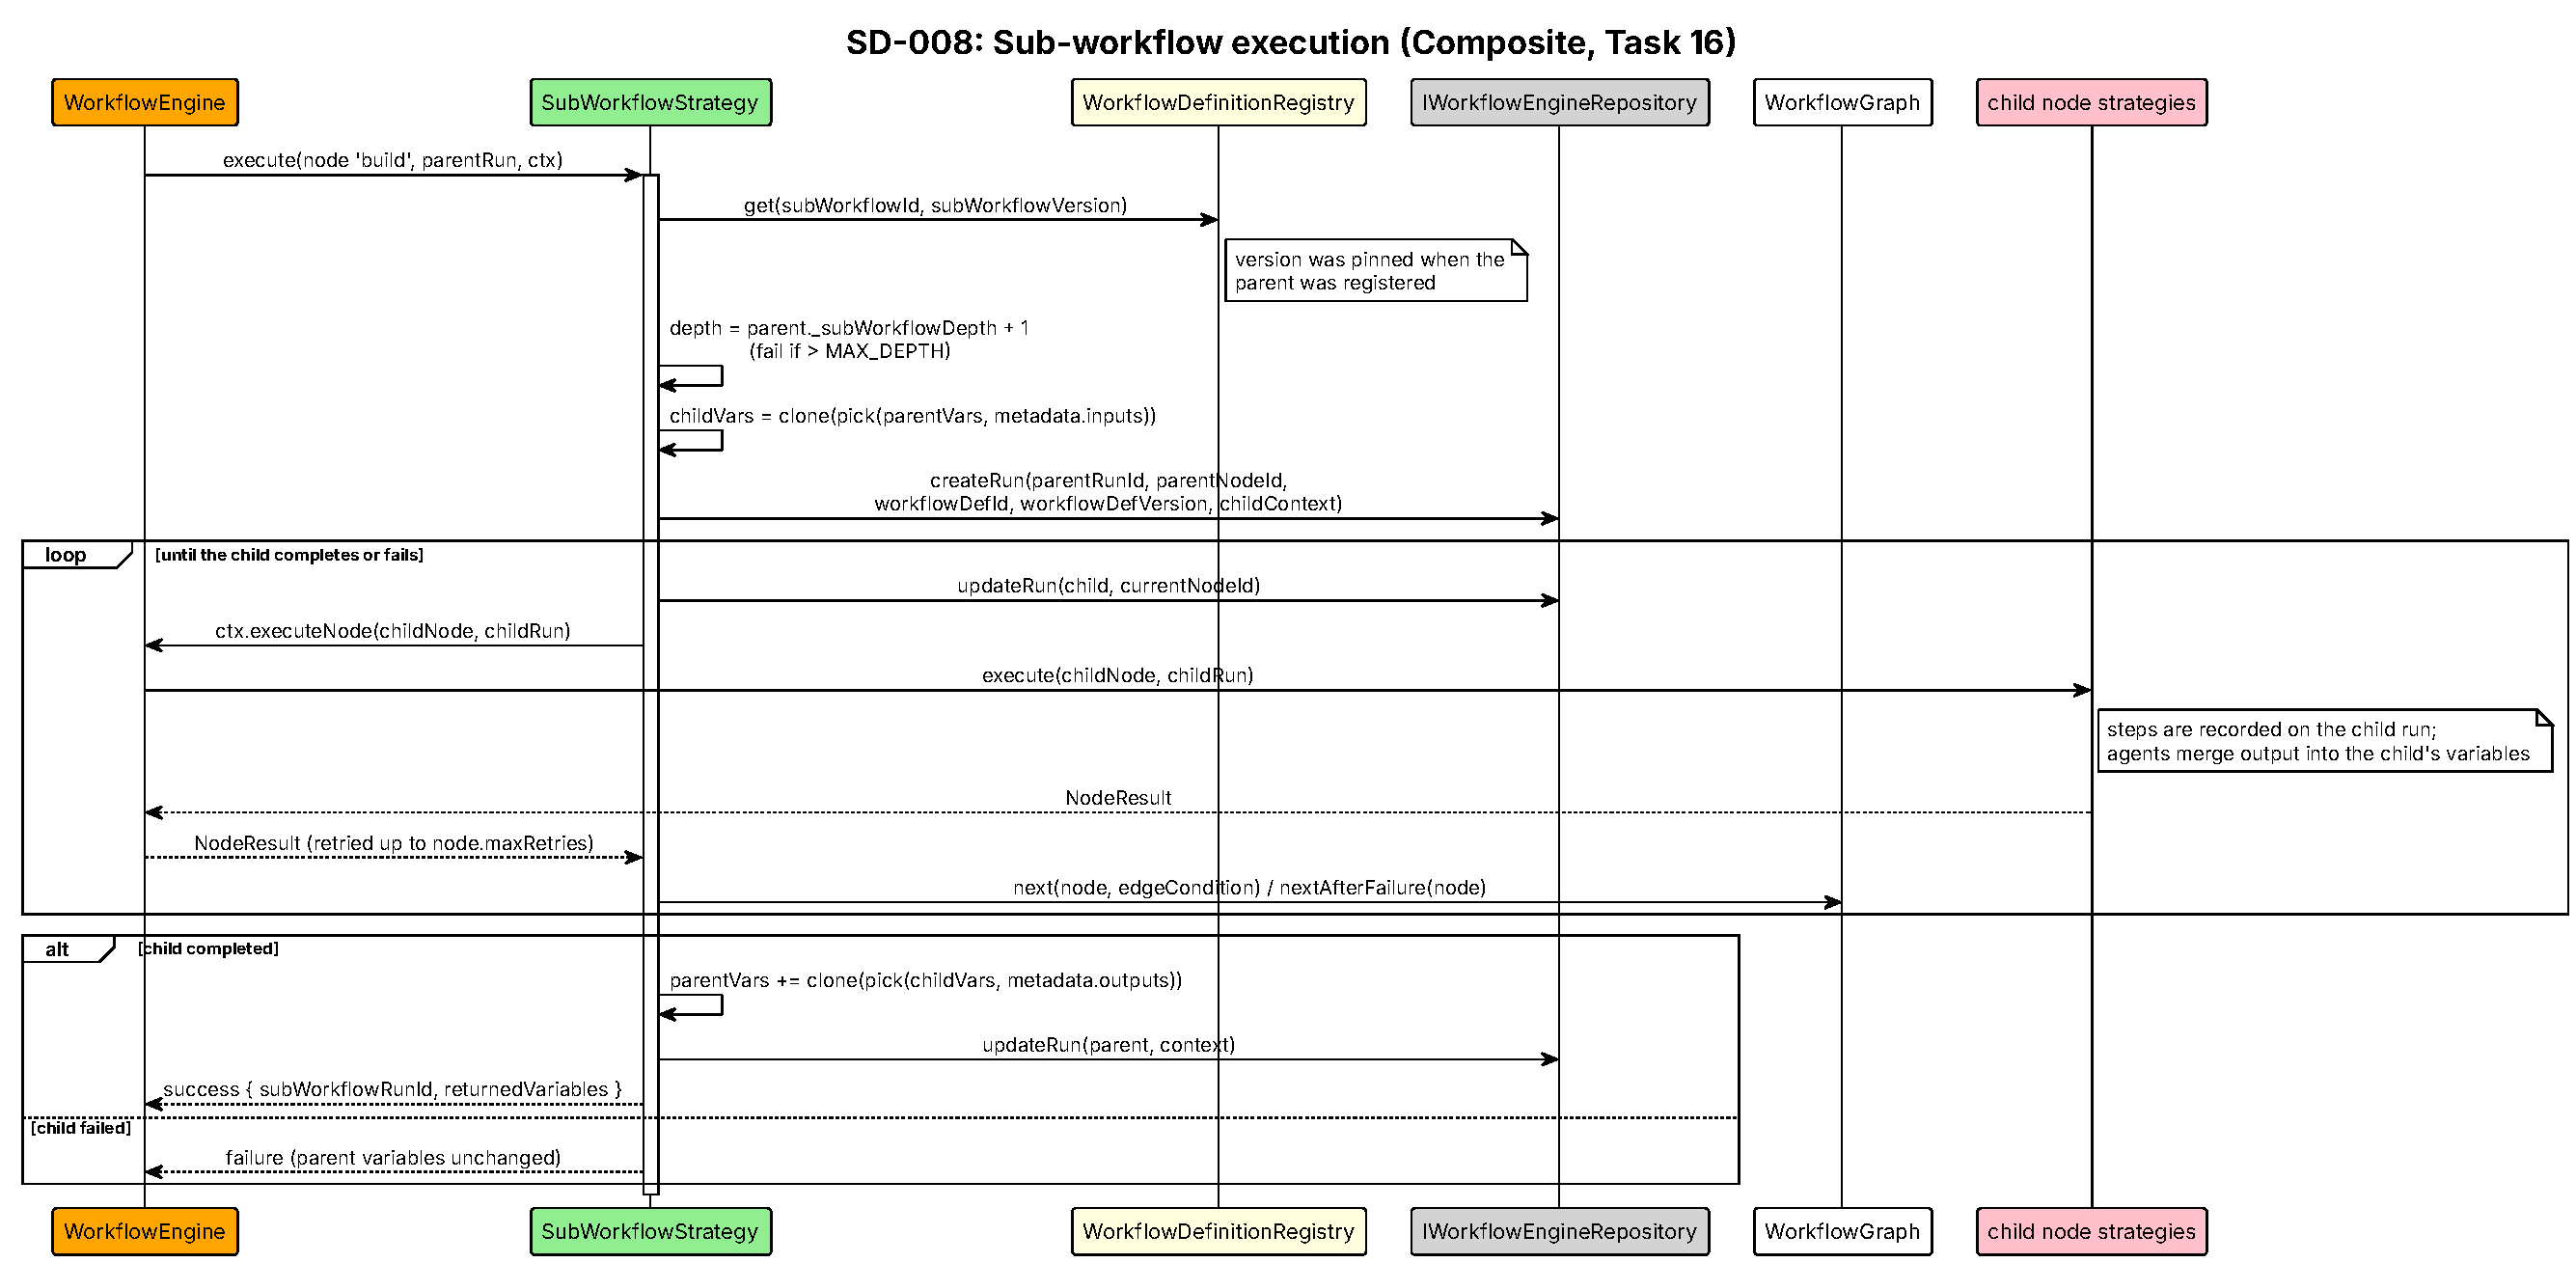
\includegraphics[width=\textwidth]{uml/SD-008-sub-workflow-execution.pdf}
\end{figure}

\begin{figure}{Sơ đồ tuần tự SD-006: ảnh chụp và khôi phục lượt chạy}
\label{fig:sd006}
\centering
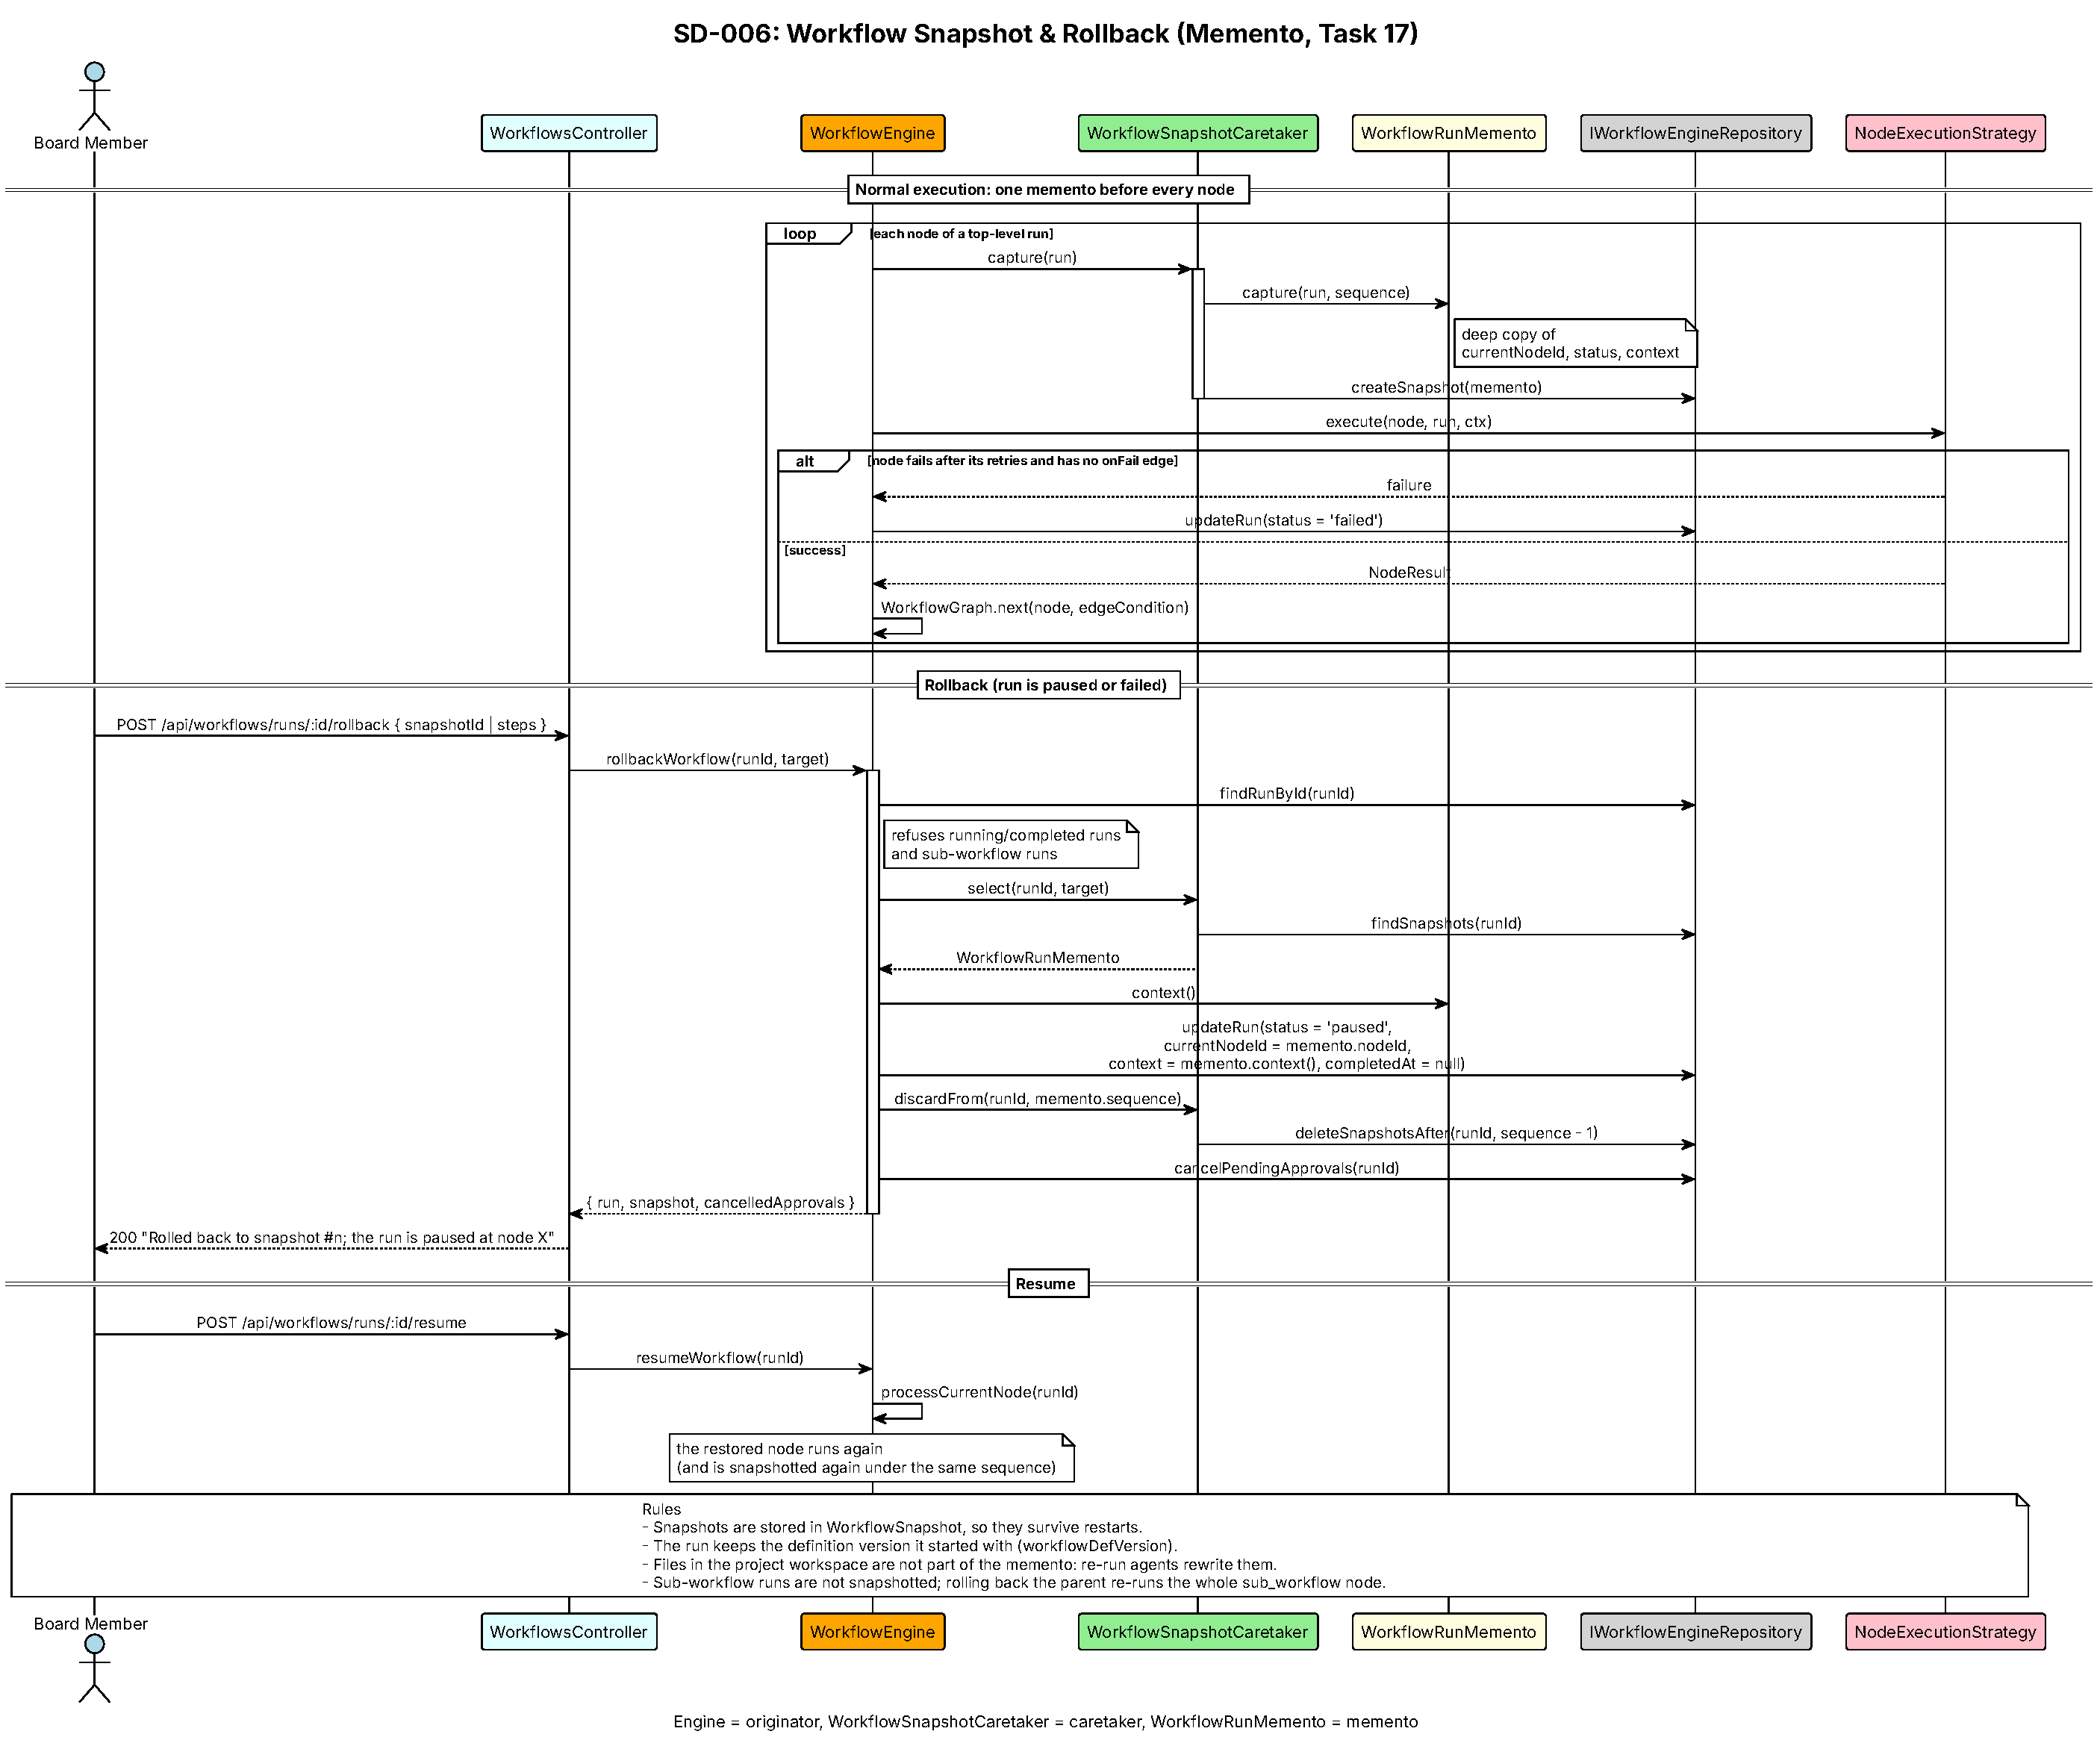
\includegraphics[width=\textwidth]{uml/SD-006-workflow-rollback.pdf}
\end{figure}

\begin{figure}{Sơ đồ tuần tự SD-009: xử lý yêu cầu có khoá API}
\label{fig:sd009}
\centering
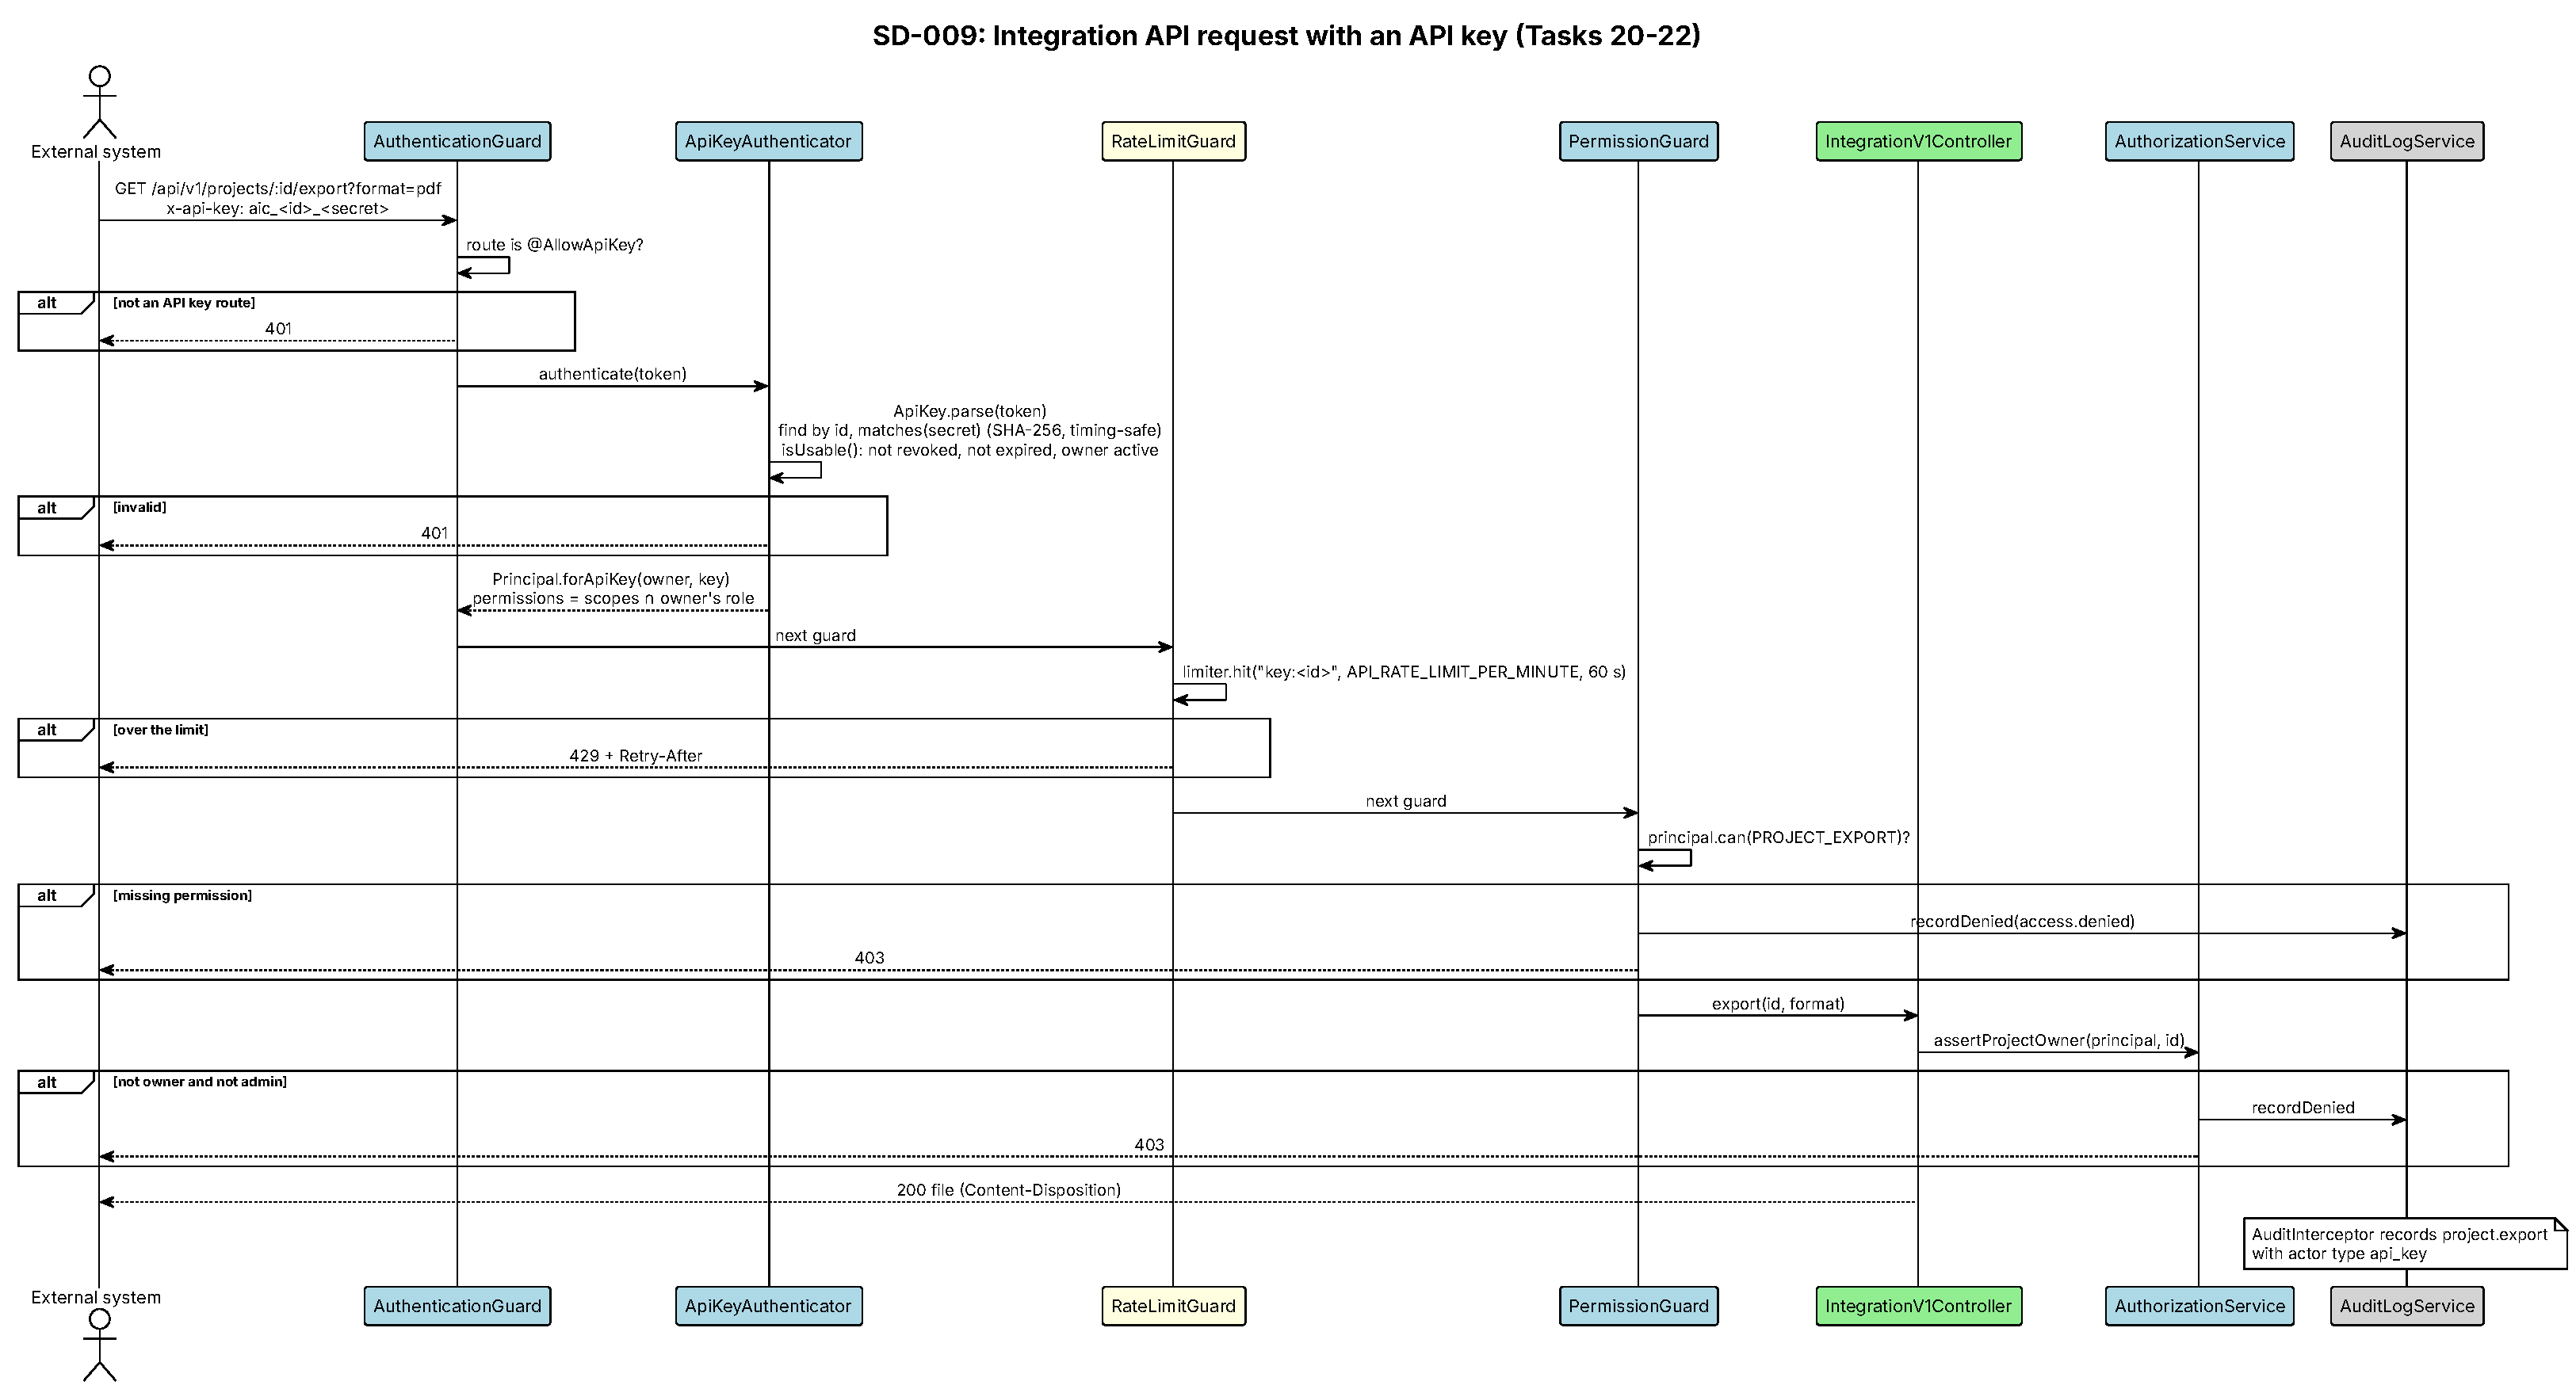
\includegraphics[width=\textwidth]{uml/SD-009-api-key-request.pdf}
\end{figure}

\begin{figure}{Sơ đồ tuần tự SD-010: gửi webhook}
\label{fig:sd010}
\centering
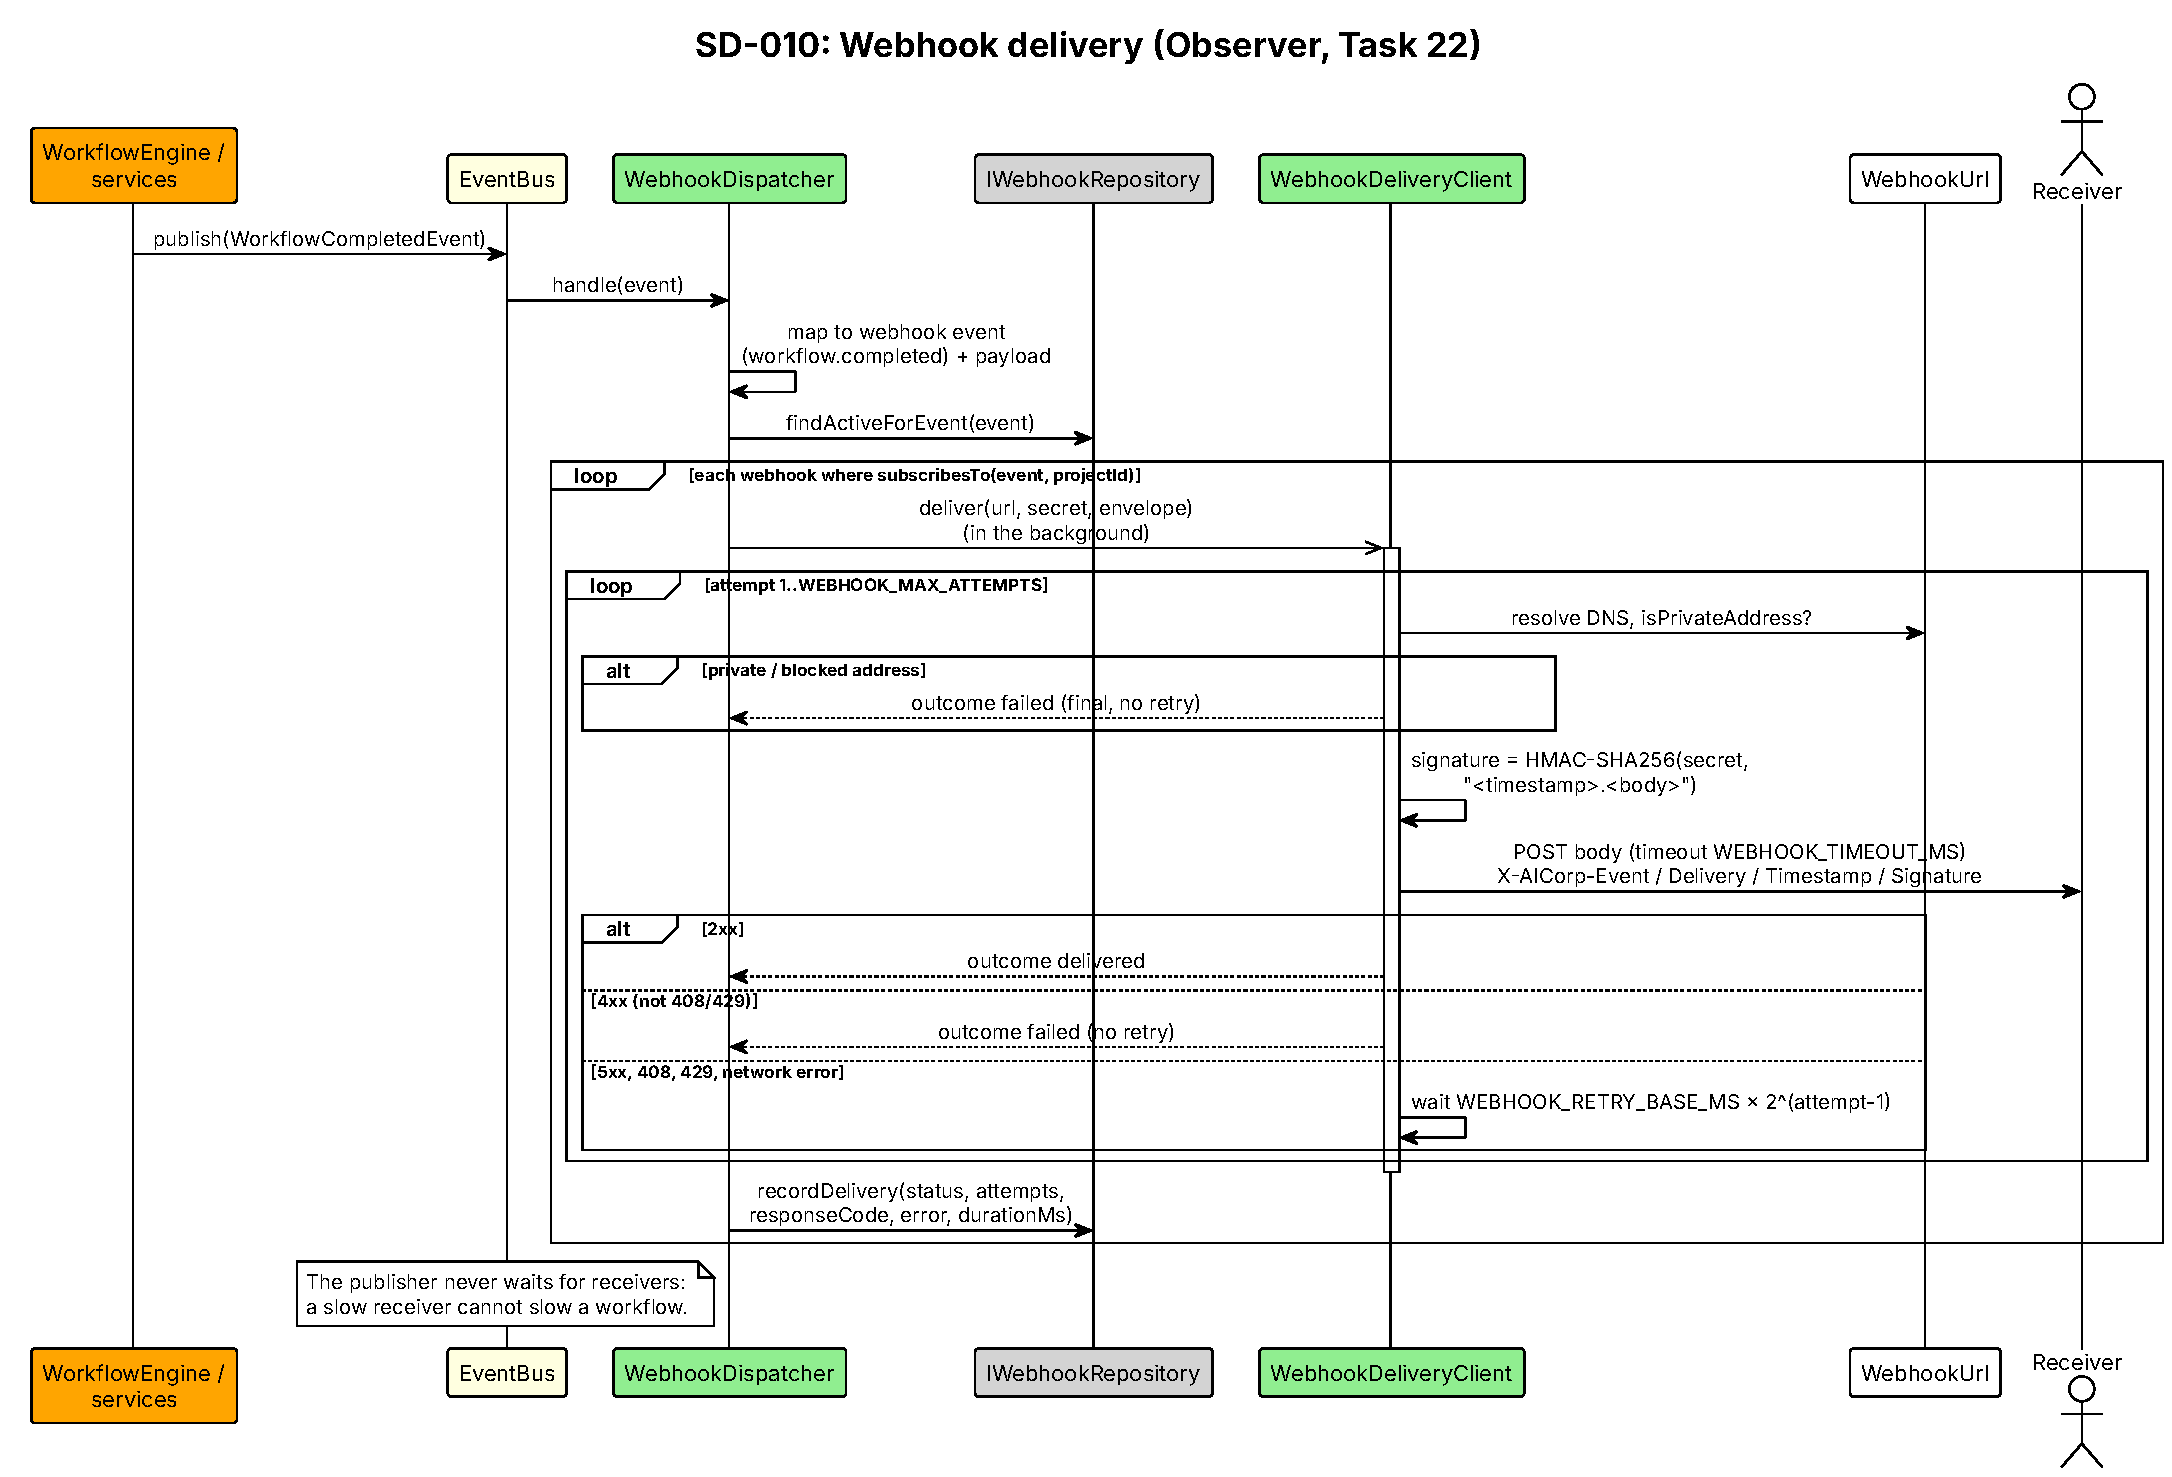
\includegraphics[width=0.9\textwidth]{uml/SD-010-webhook-delivery.pdf}
\end{figure}

\begin{figure}{Sơ đồ hoạt động AD-003: ước lượng công sức và chi phí}
\label{fig:ad003}
\centering
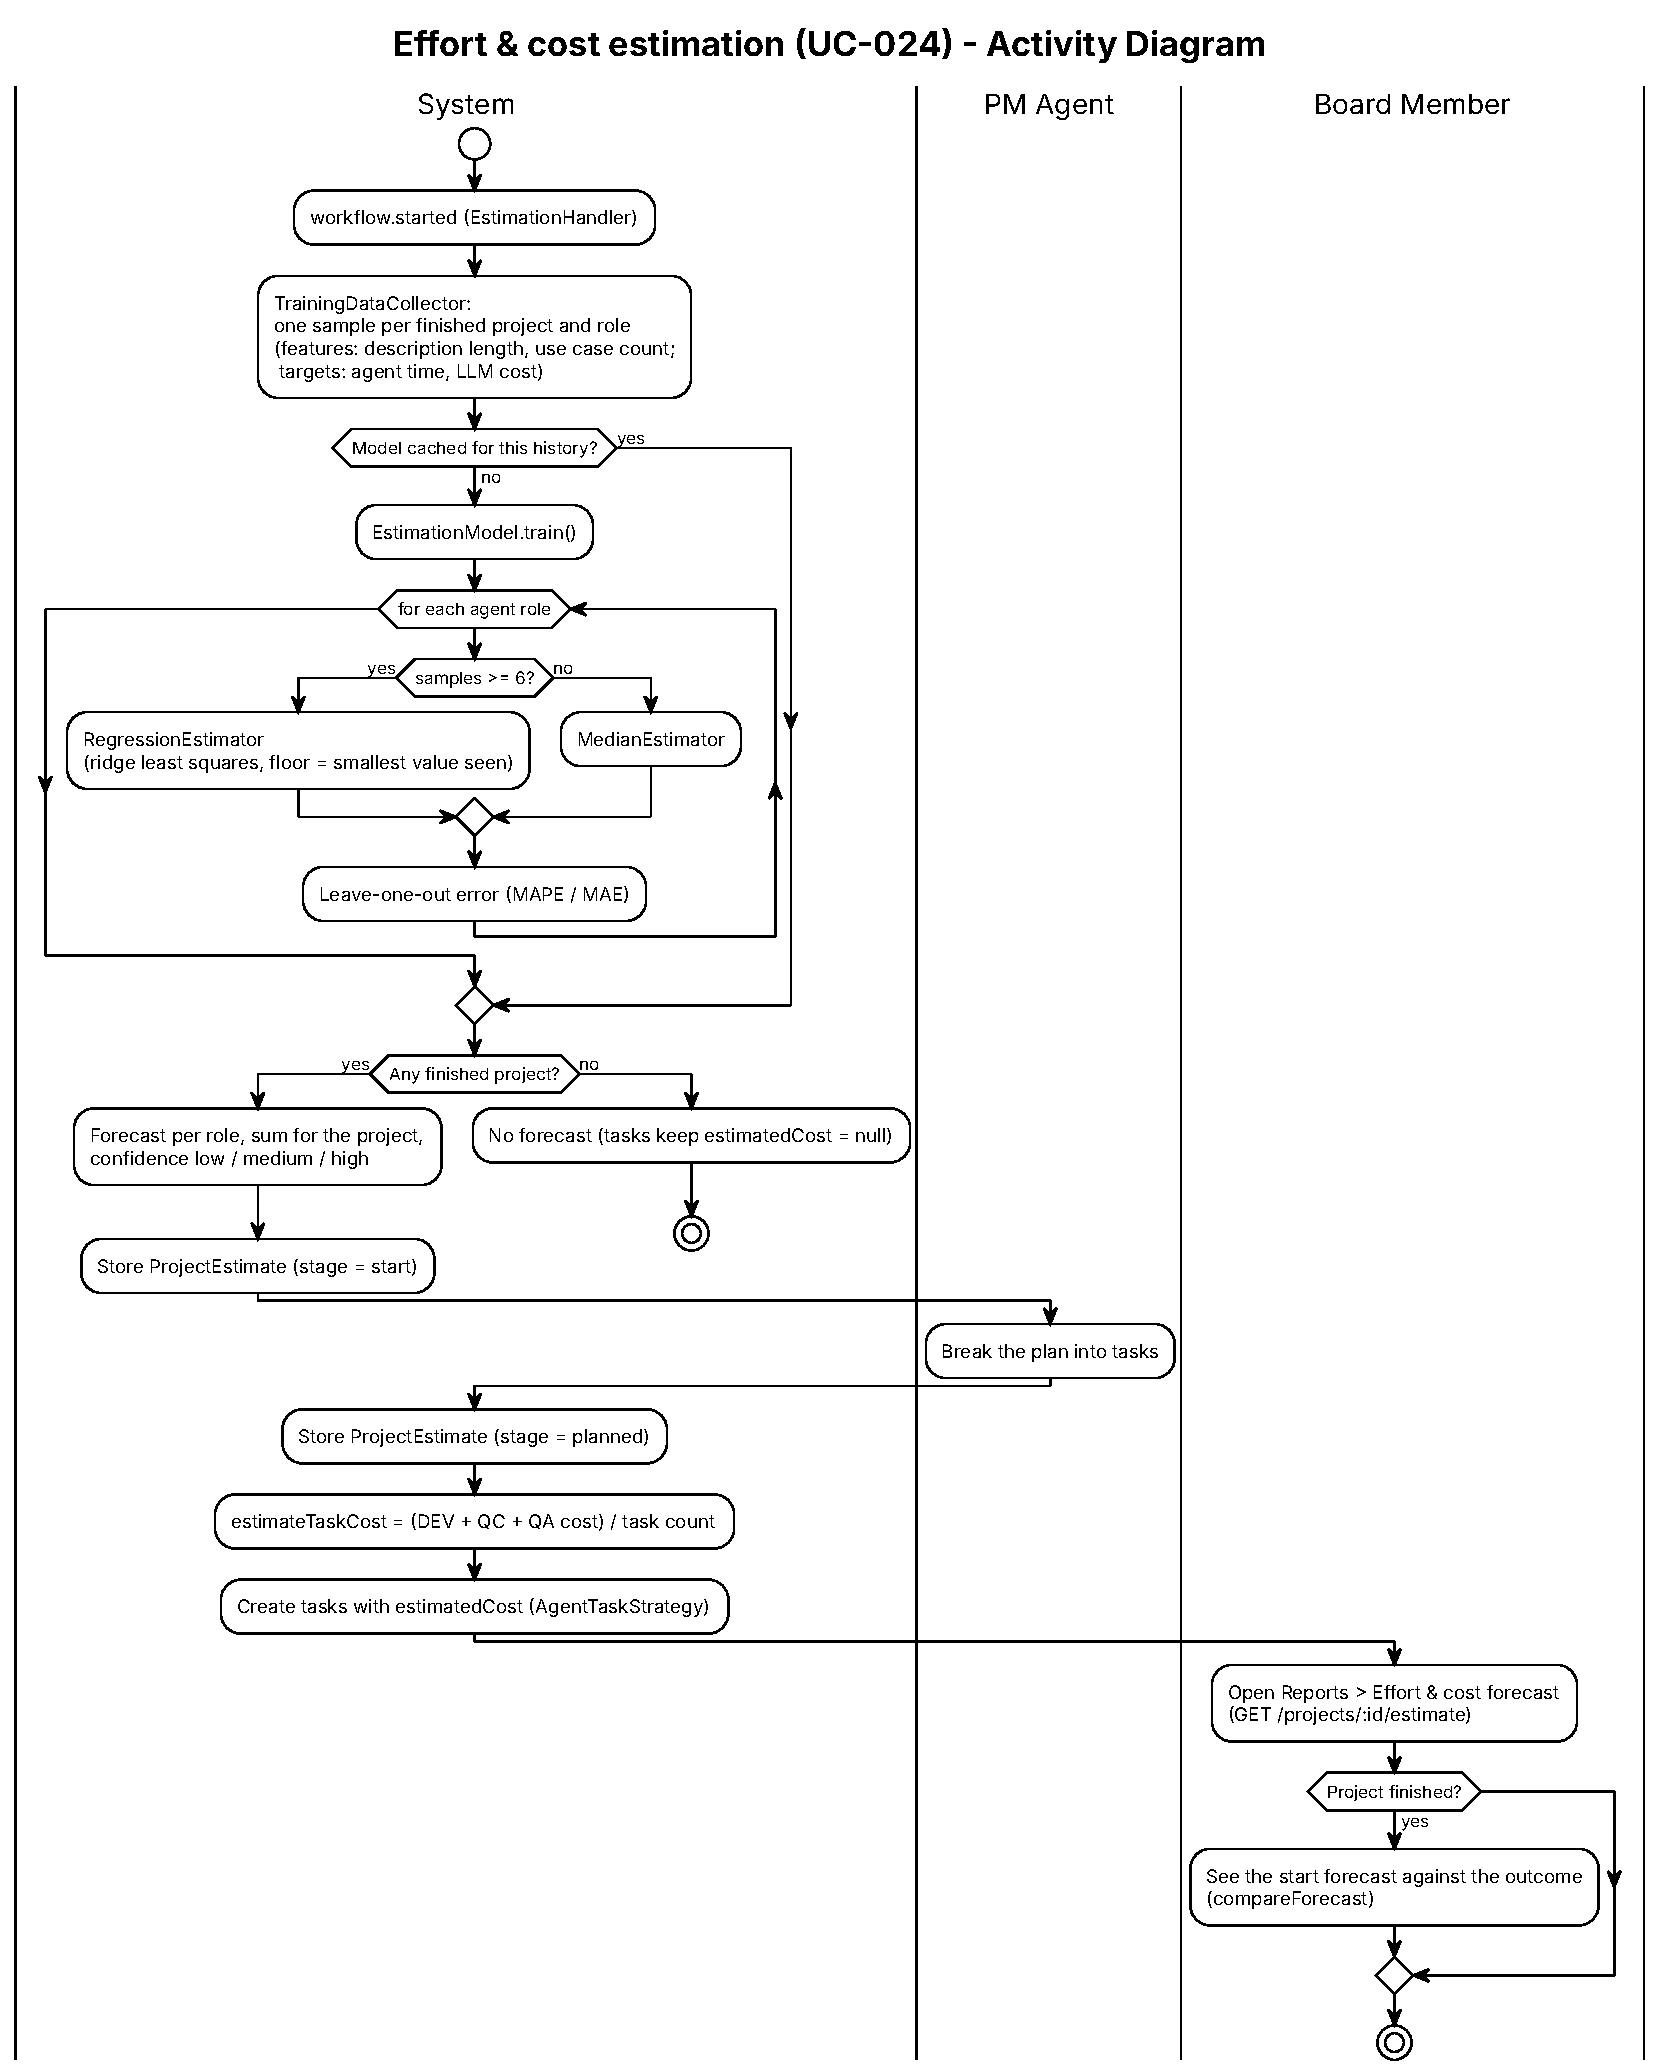
\includegraphics[height=0.55\textheight]{uml/AD-003-task-estimation-ml-pipeline.pdf}
\end{figure}

\begin{figure}{Sơ đồ hoạt động AD-004: phân tích và sửa chất lượng mã}
\label{fig:ad004}
\centering
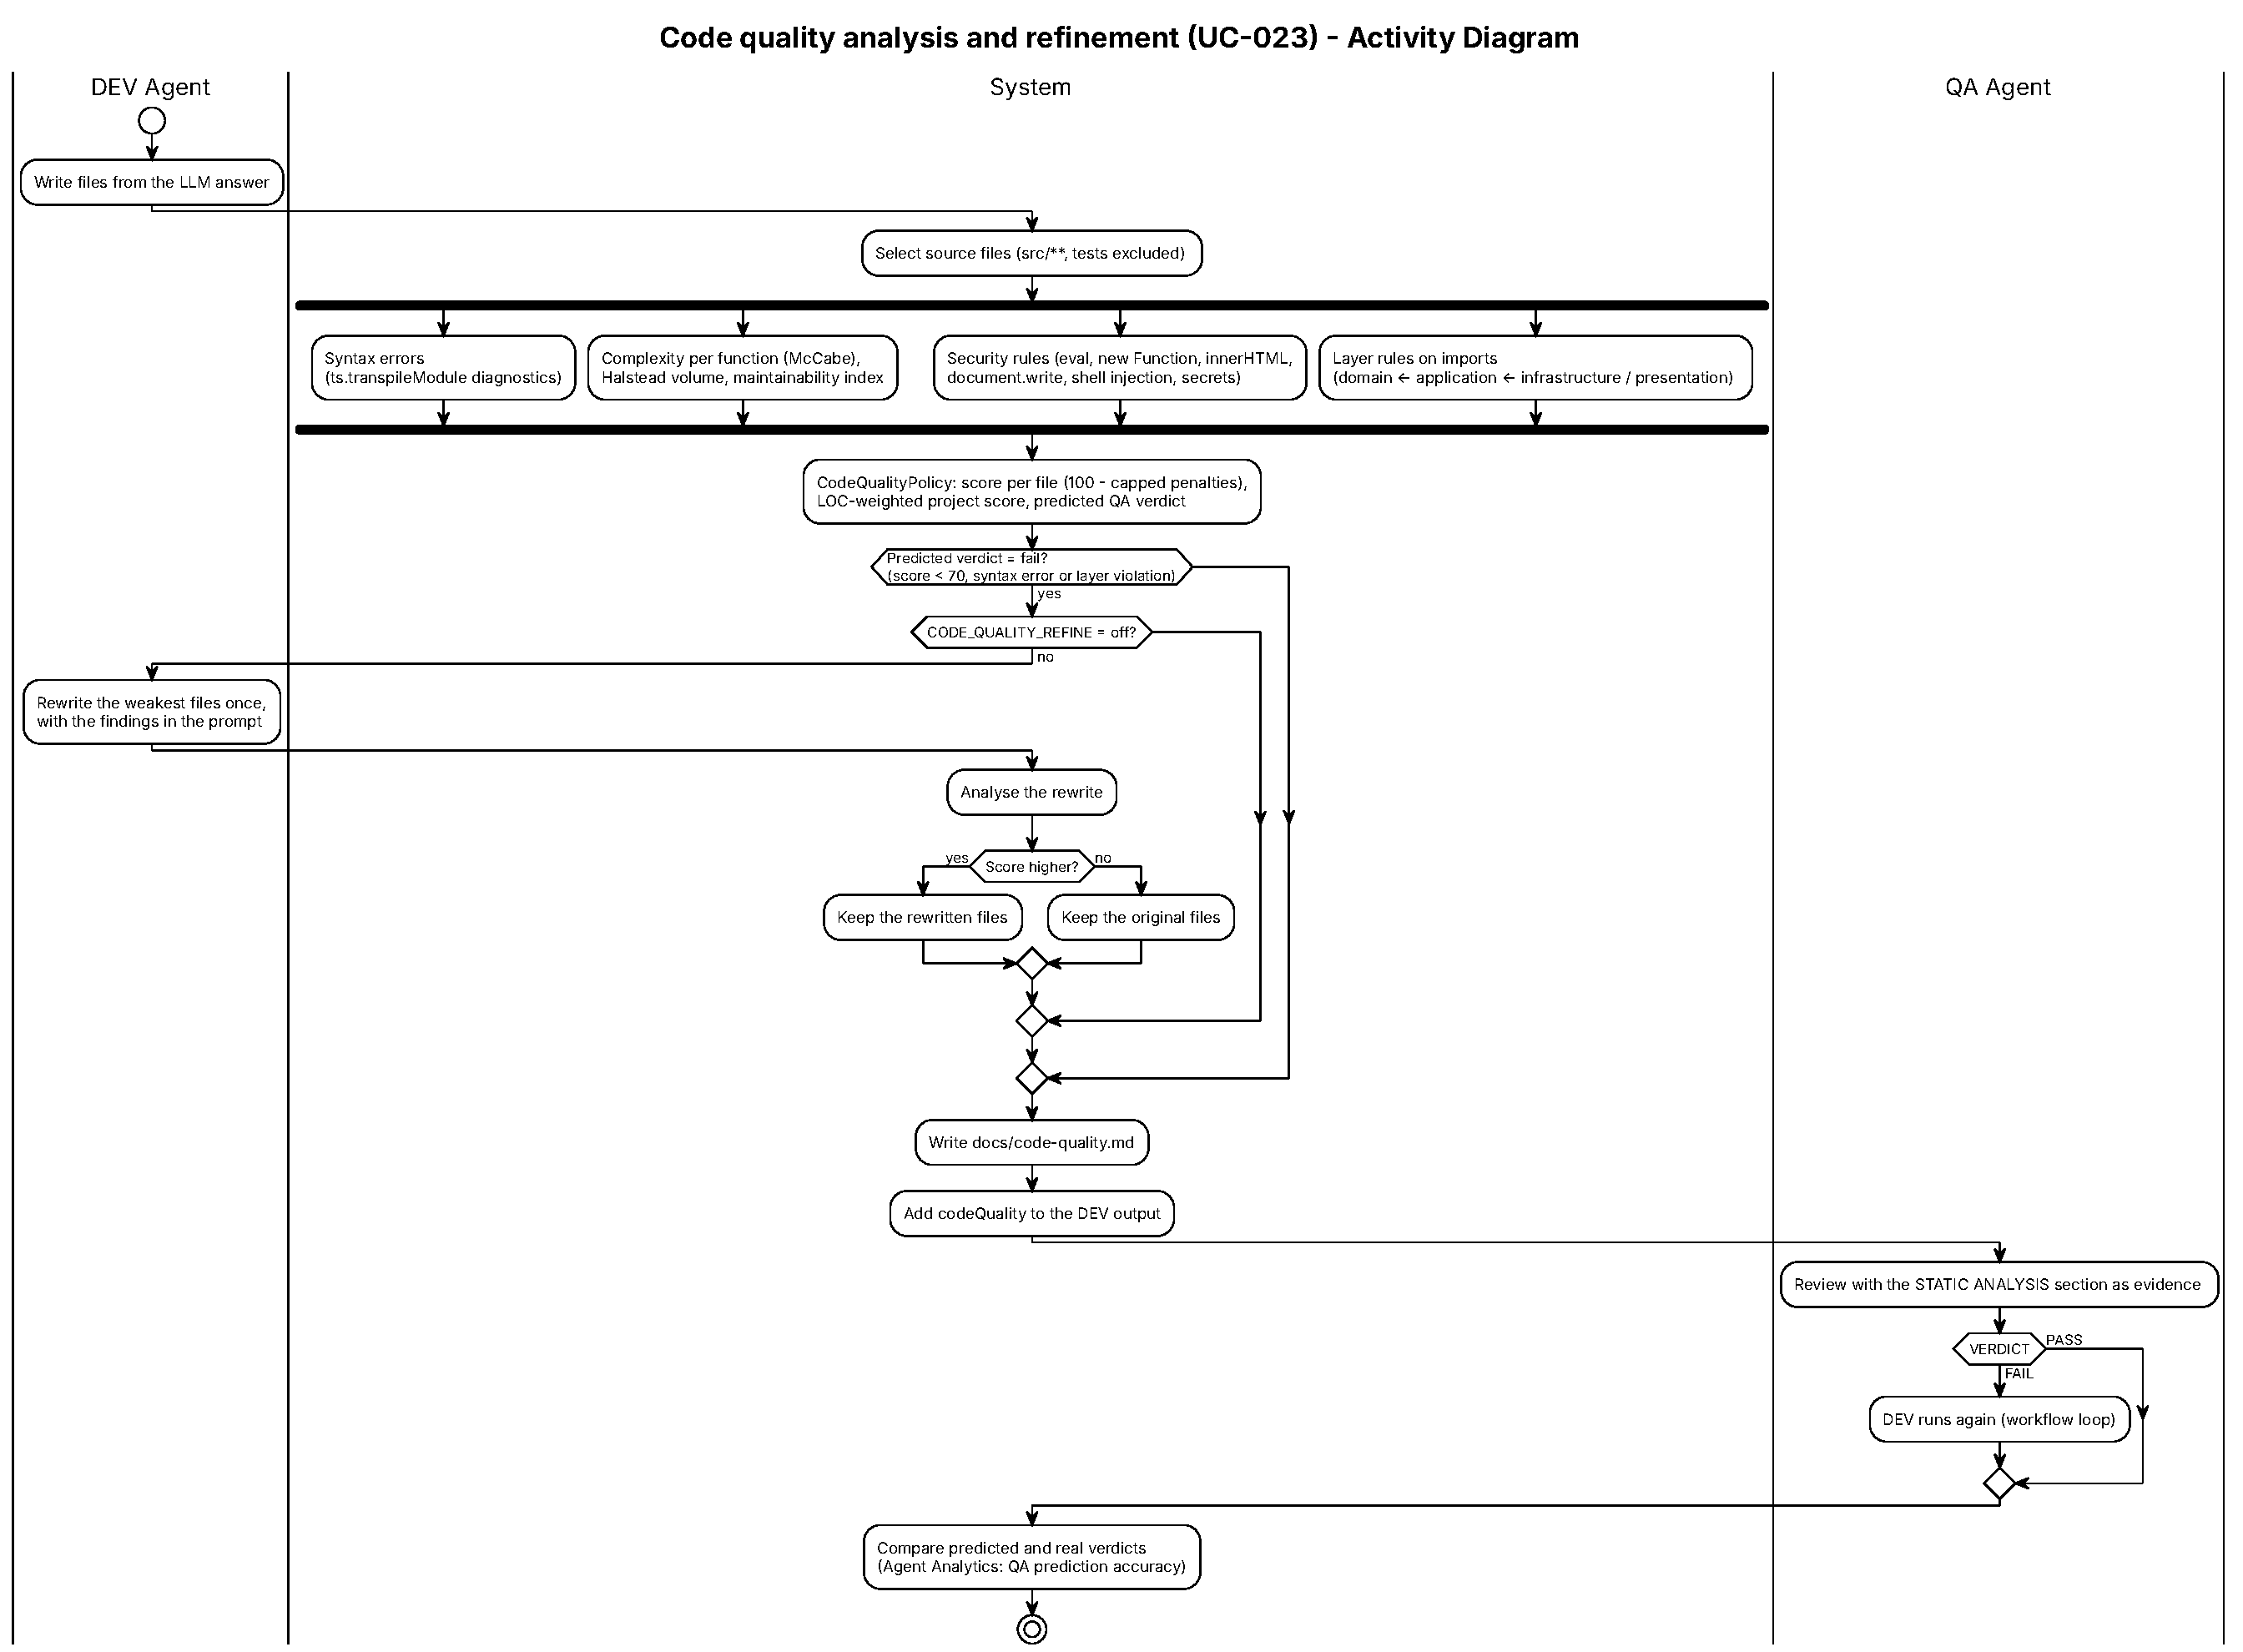
\includegraphics[width=\textwidth]{uml/AD-004-code-quality-analysis-flow.pdf}
\end{figure}

\begin{figure}{Sơ đồ máy trạng thái SM-004: phê duyệt}
\label{fig:sm004}
\centering
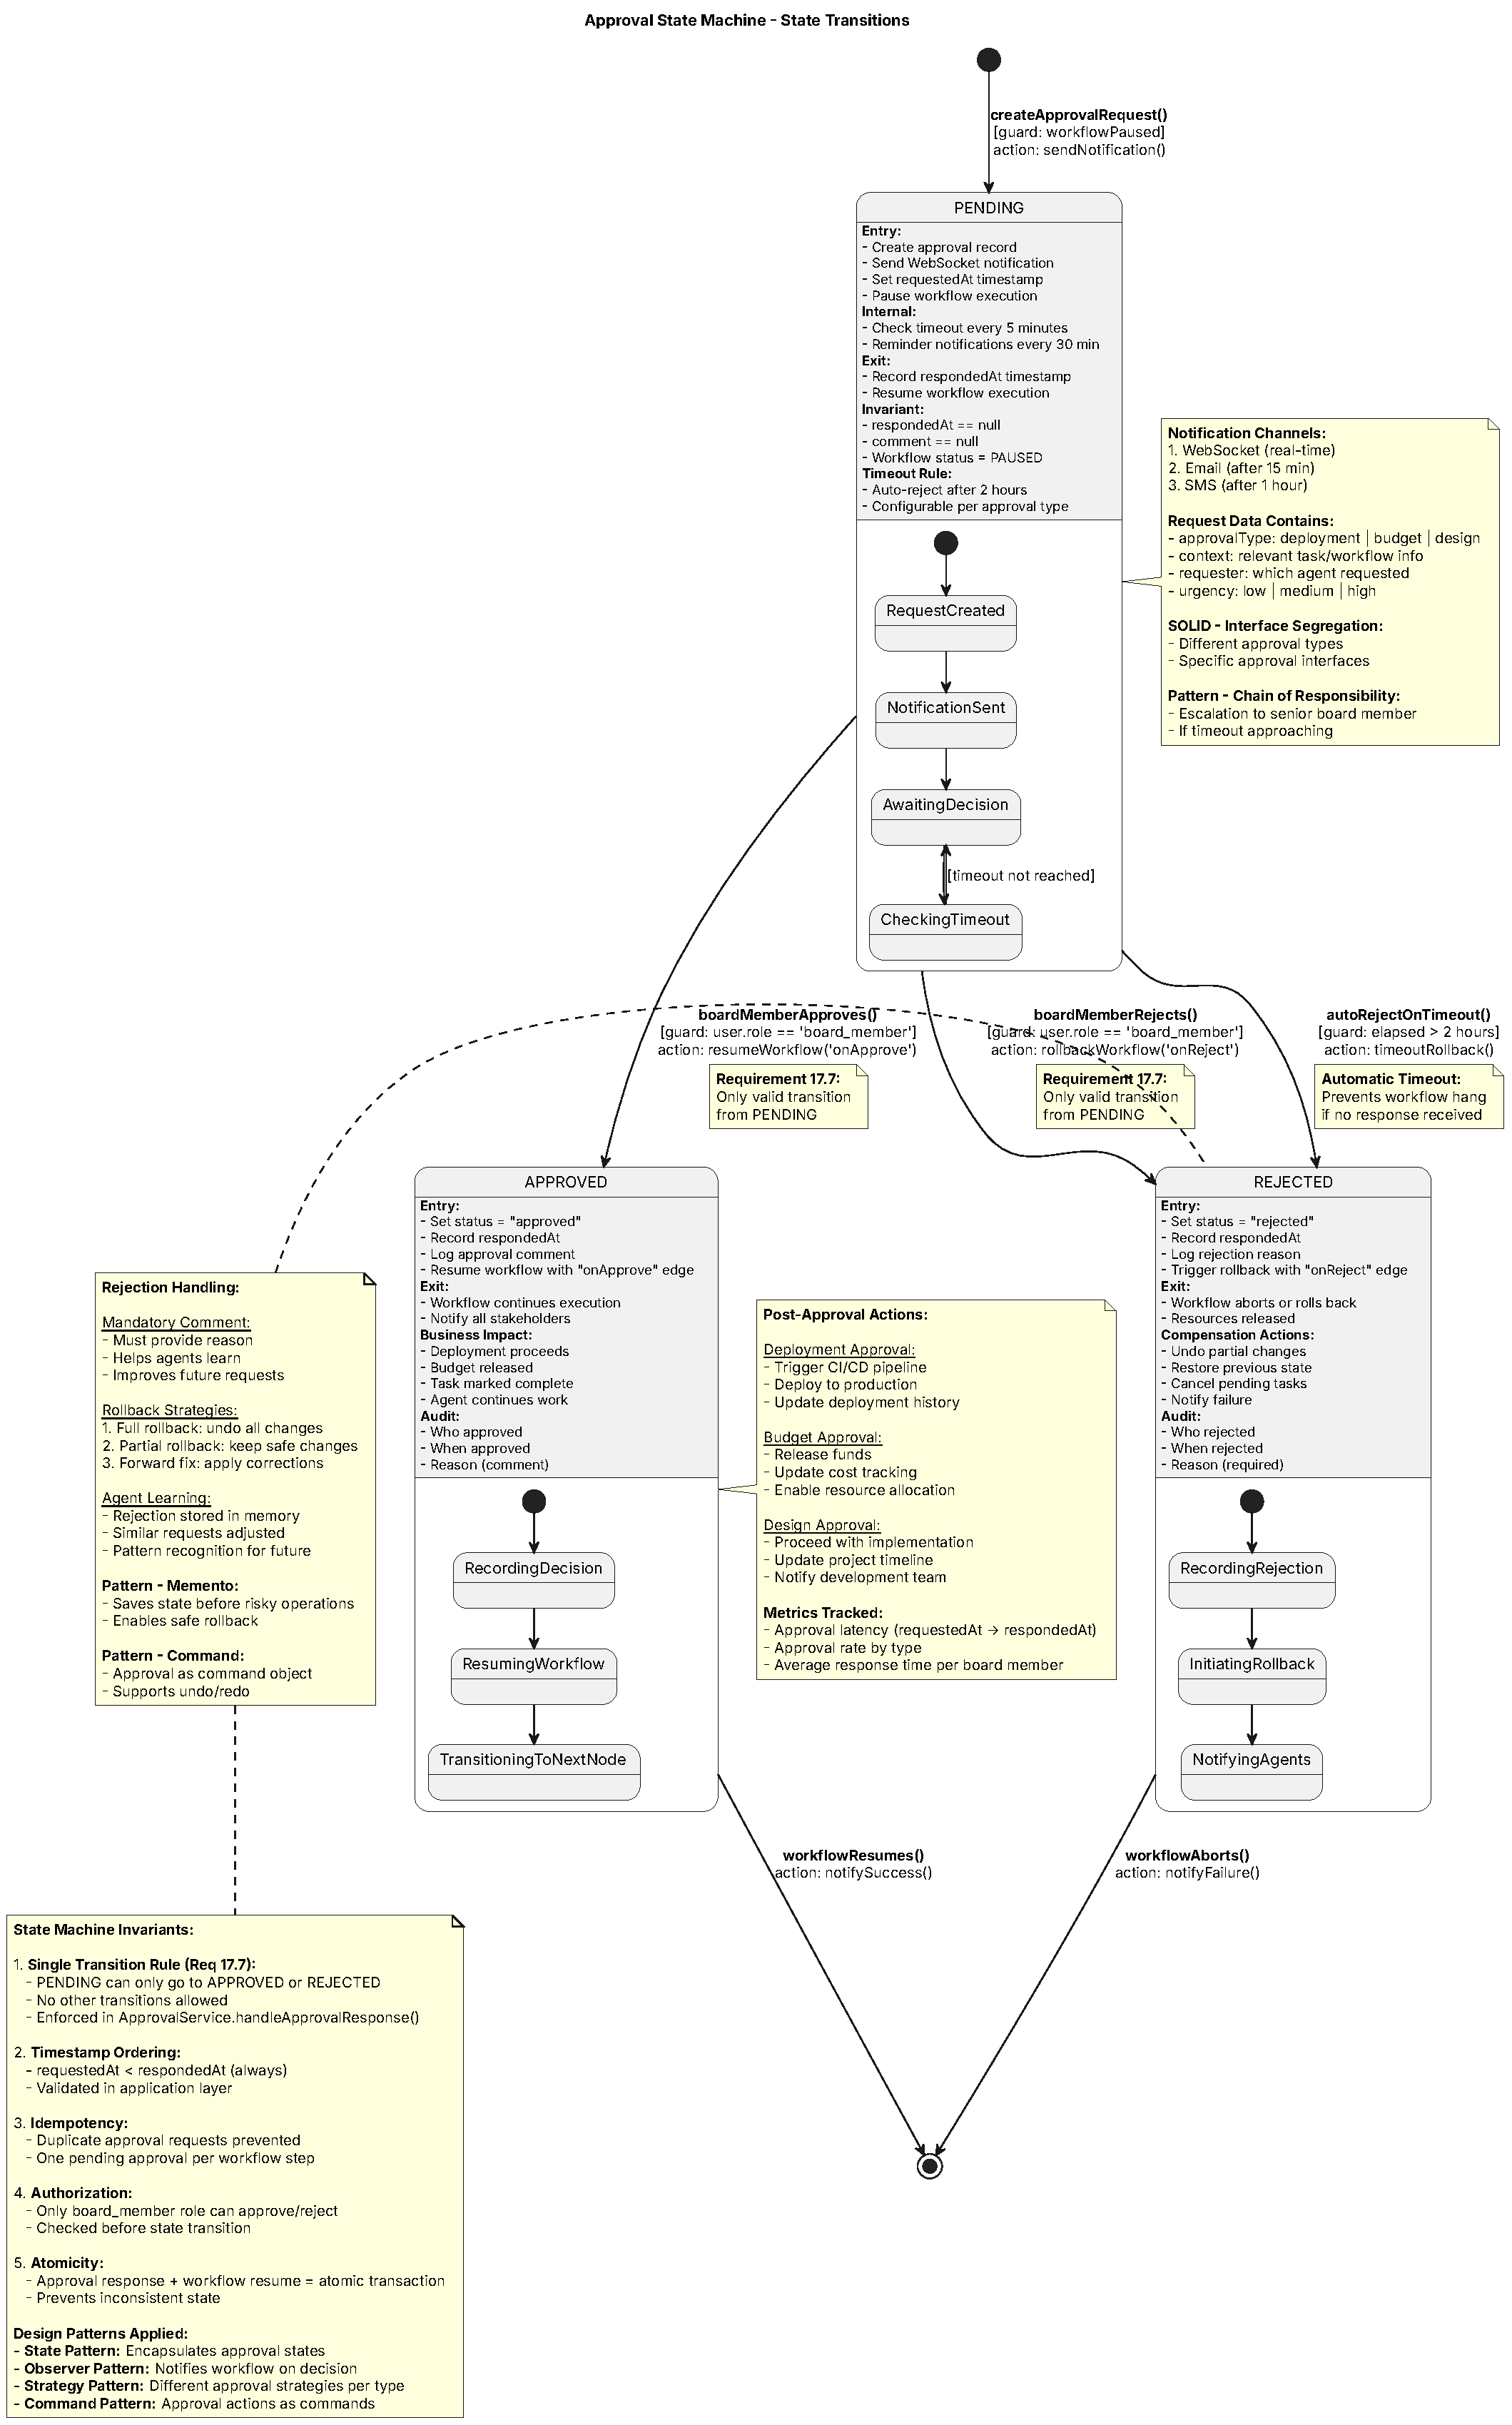
\includegraphics[height=0.5\textheight]{uml/SM-004-approval-states.pdf}
\end{figure}

\begin{figure}{Sơ đồ lớp của vòng học}
\label{fig:learning-loop}
\centering
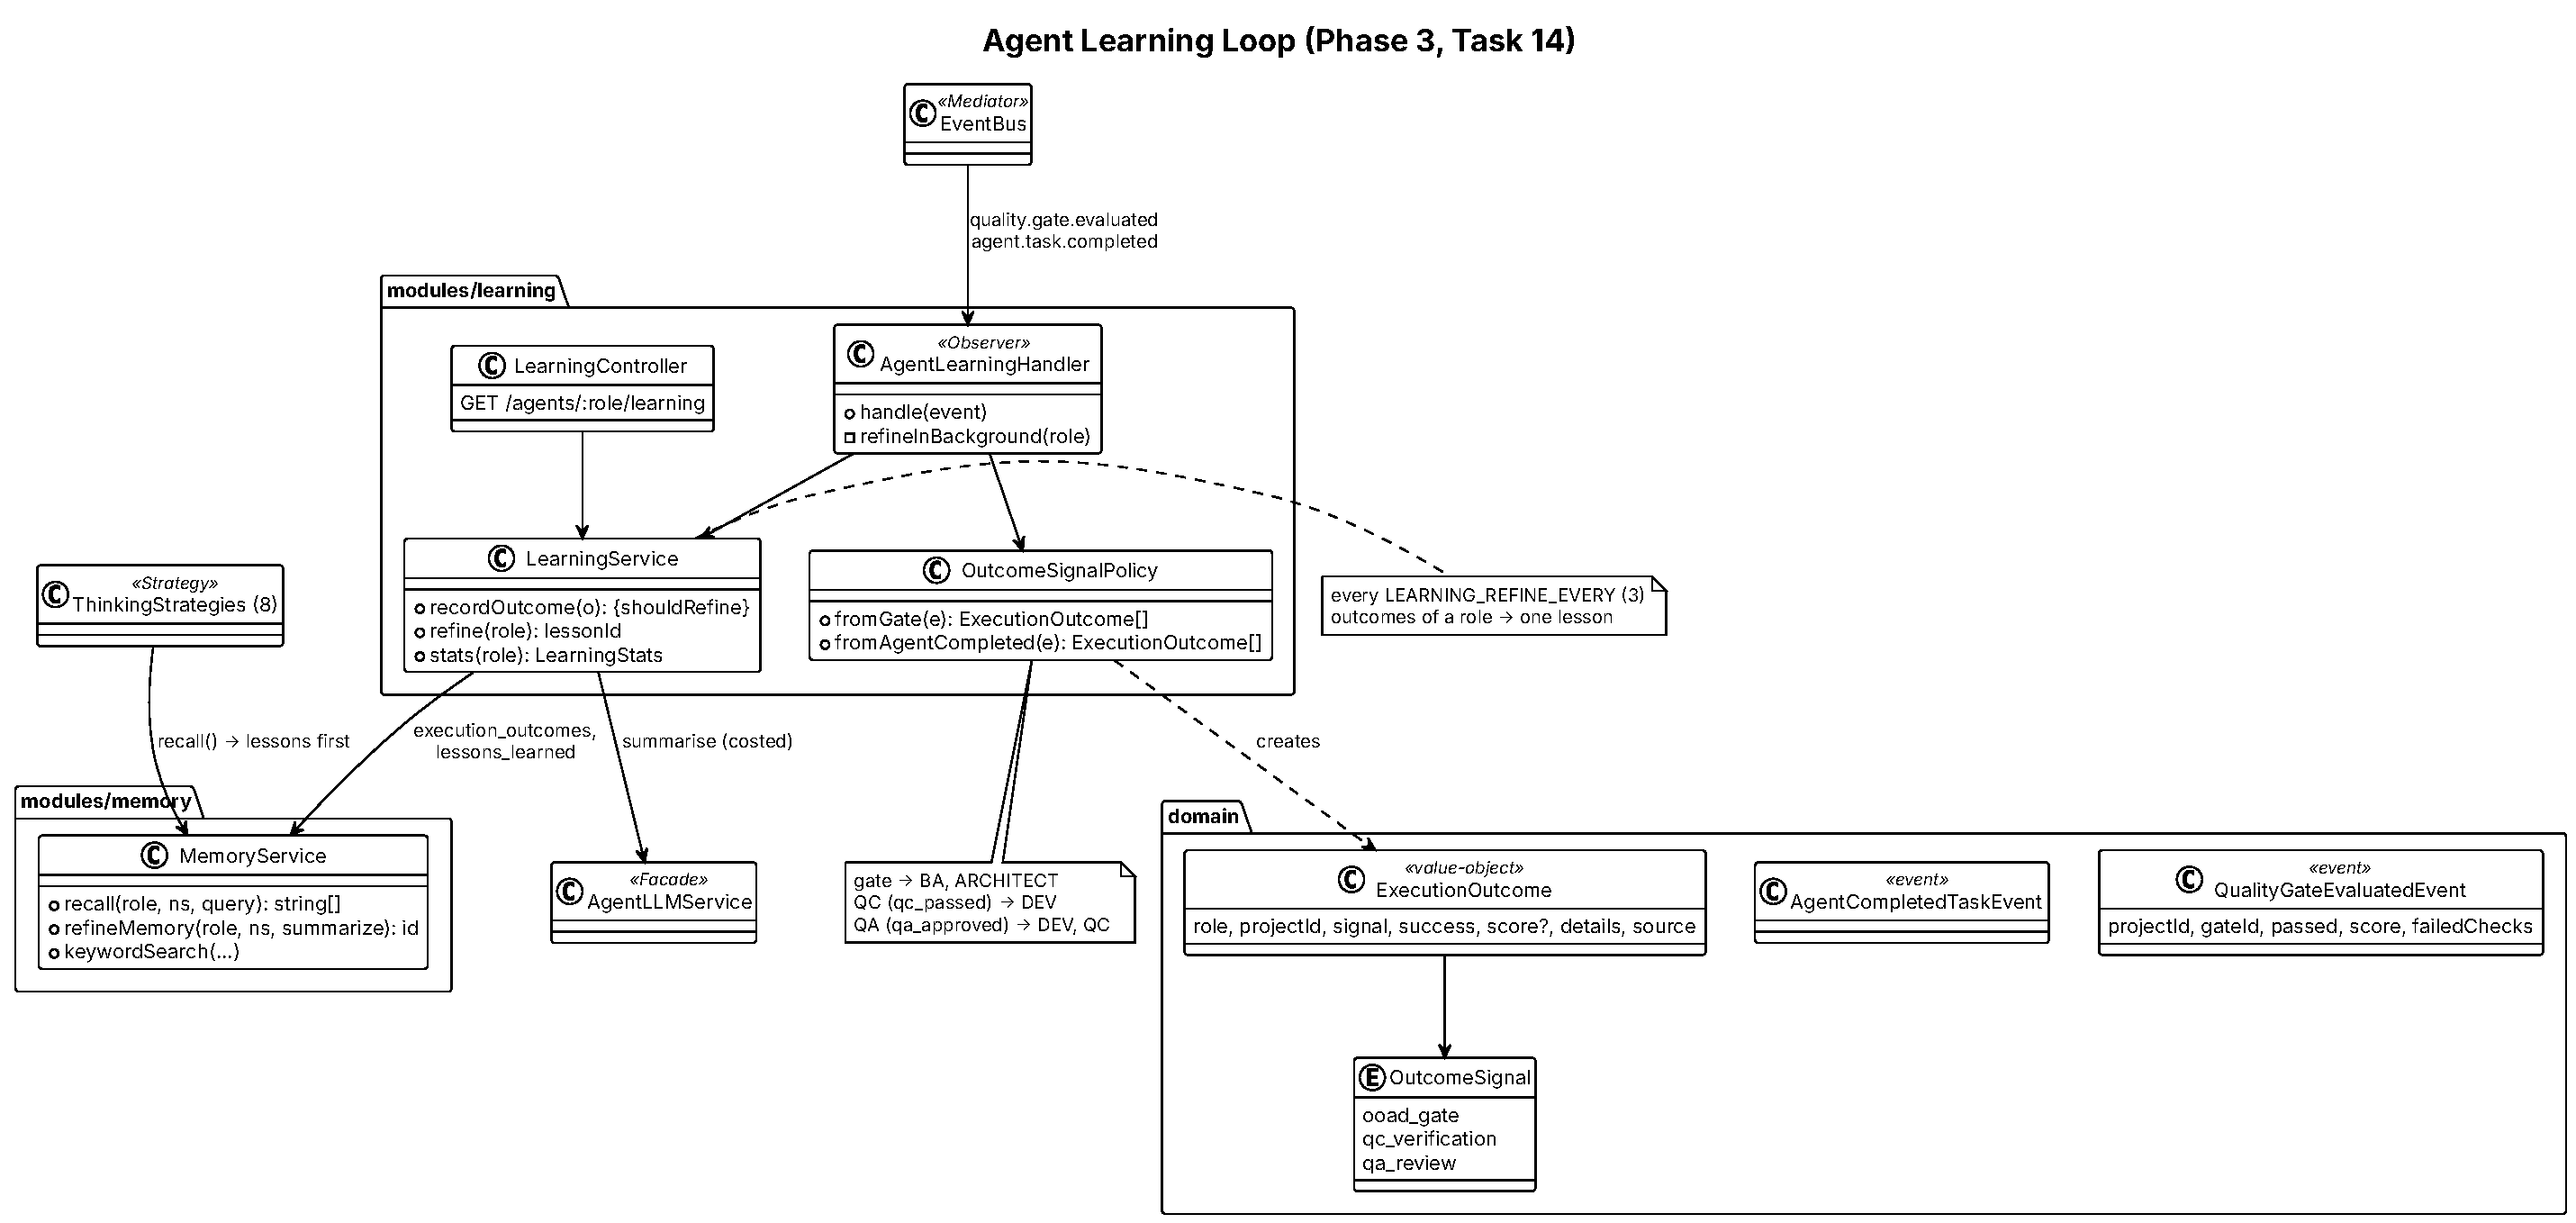
\includegraphics[width=\textwidth]{uml/learning-loop.pdf}
\end{figure}

\chapter{Giao diện lập trình}
\label{app:api}

Mọi đường dẫn đều có tiền tố \code{/api}. Trừ \code{auth/register}, \code{auth/login} và \code{health}, mọi route đều đòi JWT (giao diện web) hoặc khoá API (nhóm \code{/v1}) và được kiểm tra quyền theo vai trò. Khi \code{ENABLE_SWAGGER=true}, tài liệu OpenAPI đầy đủ có tại \code{/api/docs}.

\begin{table}{Các nhóm route của API}
\label{tab:api}
\footnotesize
\begin{tabularx}{\textwidth}{|P{2.6cm}|L|}
\hline
\textbf{Nhóm} & \textbf{Route} \\ \hline
Xác thực & \code{POST auth/register}, \code{POST auth/login}, \code{GET auth/me} \\ \hline
Dự án & \code{GET/POST projects}, \code{GET/PATCH/DELETE projects/:id} (\code{PATCH} với trạng thái tạm dừng, tiếp tục, huỷ tác động lên lượt chạy mới nhất), \code{POST projects/:id/workflow/start} \\ \hline
Công việc, mốc & \code{GET tasks}, \code{POST projects/:projectId/tasks}, \code{PATCH tasks/:id}; \code{GET/POST projects/:projectId/milestones}, \code{PATCH milestones/:id} \\ \hline
Sản phẩm dự án & \code{GET projects/:id/files}, \code{GET projects/:id/files/*}, \code{GET projects/:id/archive} (zip), \code{GET projects/:id/quality-gates} \\ \hline
Phê duyệt & \code{GET approvals}, \code{POST approvals/:id/approve}, \code{POST approvals/:id/reject} (bắt buộc lý do; 409 nếu đã trả lời) \\ \hline
Quy trình & \code{GET workflows/templates}, \code{POST workflows/templates/:templateId/preview}, \code{GET workflows/definitions[/:definitionId]}, \code{GET workflows/runs/:runId}, \code{GET workflows/runs/:runId/snapshots}, \code{POST workflows/runs/:runId/rollback}, \code{POST workflows/runs/:runId/pause}, \code{POST workflows/runs/:runId/resume} \\ \hline
Mô hình LLM & \code{GET models}, \code{GET models/available}, \code{PATCH models/:role} (kèm \code{providerId}) \\ \hline
Nhà cung cấp LLM & \code{GET/POST llm-providers}, \code{GET llm-providers/kinds}, \code{PATCH/DELETE llm-providers/:id}, \code{POST llm-providers/:id/test}, \code{GET llm-providers/:id/remote-models}, \code{POST llm-providers/:id/models}, \code{PATCH/DELETE llm-providers/:id/models/:modelId} \\ \hline
Chi phí, báo cáo, xuất & \code{GET cost/summary}, \code{GET reports/projects/:id/cost}, \code{GET reports/performance}, \code{POST reports/weekly/run}, \code{GET projects/:id/export?format=json|csv|pdf} \\ \hline
Phân tích, dự báo, chất lượng & \code{GET analytics/agents}, \code{GET agents/:role/learning}, \code{GET projects/:id/estimate}, \code{GET analytics/estimation}, \code{GET projects/:id/code-quality}, \code{GET ooad-metrics/dashboard}, \code{GET ooad-metrics/project/:id}, \code{GET ooad-metrics/leaderboard} \\ \hline
Người dùng, kiểm toán & \code{GET users}, \code{GET users/roles}, \code{PATCH users/:id/role}, \code{PATCH users/:id/active}; \code{GET audit}, \code{GET audit/export}, \code{GET audit/anomalies} \\ \hline
Tích hợp (quản trị) & \code{GET integrations/events}, \code{GET/POST integrations/api-keys}, \code{DELETE integrations/api-keys/:id}, \code{GET/POST integrations/webhooks}, \code{DELETE integrations/webhooks/:id}, \code{POST integrations/webhooks/:id/test}, \code{GET integrations/webhooks/:id/deliveries} \\ \hline
API công khai (khoá API) & \code{GET/POST v1/projects}, \code{GET v1/projects/:id/status}, \code{GET v1/projects/:id/reports/cost}, \code{GET v1/projects/:id/export}, \code{GET/POST v1/webhooks}, \code{DELETE v1/webhooks/:id} \\ \hline
Sức khoẻ & \code{GET health} (503 khi cơ sở dữ liệu ngừng), \code{GET health/live} \\ \hline
\end{tabularx}
\end{table}

Về WebSocket (Socket.IO, xác thực bằng JWT lúc kết nối): máy khách gửi \code{subscribe_project} để nhận \code{project_event} của một dự án; máy chủ phát thêm \code{system_event} (trạng thái tác tử) và \code{user_event}. Thông điệp \code{human:approval_response} bị từ chối; phê duyệt chỉ đi qua REST.

\chapter{Tái tạo số liệu kiểm thử và hiệu năng}
\label{app:tai-tao}

\section{Kiểm thử tự động}

\begin{Verbatim}
pnpm install
cd apps/api && npx jest              # 50 bộ, 707 đạt, 15 bỏ qua
cd apps/api && npm run test:cov      # độ bao phủ, lỗi nếu dưới ngưỡng
cd apps/web && npx vitest run && npx tsc --noEmit
\end{Verbatim}

\section{Kiểm thử đầu cuối}

Mỗi lần chạy có script, kết quả và ảnh chụp màn hình lưu trong một thư mục \code{docs/*-e2e/} của kho mã, kèm README ghi môi trường và câu lệnh. Script in một dòng cho mỗi kiểm tra và trả mã 1 nếu có kiểm tra hỏng. Môi trường chung gồm PostgreSQL 16 có pgvector, Redis 7, API build ở chế độ production và LLM kịch bản \code{scripts/demo/demo-llm.cjs} (tương thích OpenAI, cổng 20128). Lần chạy triển khai đi qua nginx với cấu hình giống \code{apps/web/nginx.conf}.

\begin{table}{Script của các lần chạy đầu cuối}
\label{tab:e2e-script}
\small
\begin{tabularx}{\textwidth}{|L|P{6.2cm}|r|}
\hline
\textbf{Lần chạy} & \textbf{Script} & \textbf{Kiểm tra} \\ \hline
Triển khai và trình diễn & \code{docs/phase7-e2e/e2e.mjs} sau \code{scripts/demo/seed-demo.mjs} & 24 \\ \hline
Phân tích, dự báo, chất lượng mã & \code{docs/phase6-e2e/e2e.mjs} & 21 \\ \hline
Bảo mật, kiểm toán, tích hợp & \code{docs/phase5-e2e/e2e.mjs} & 44 \\ \hline
Bộ máy quy trình & \code{docs/phase4-e2e/e2e.mjs} & theo kịch bản \\ \hline
\end{tabularx}
\end{table}

\section{LLM kịch bản}

Máy chủ trả lời theo vai trò và nội dung lời nhắc. Bảng~\ref{tab:kich-ban} liệt kê các quy tắc ảnh hưởng tới kết quả đánh giá.

\begin{table}{Quy tắc của LLM kịch bản}
\label{tab:kich-ban}
\small
\begin{tabularx}{\textwidth}{|P{5cm}|L|}
\hline
\textbf{Điều kiện} & \textbf{Câu trả lời} \\ \hline
Tên dự án bắt đầu bằng ``Legacy'' & Mã lần đầu của DEV nhập hạ tầng từ miền, có khoá viết cứng, \code{eval} và phương thức dài, còn bản sửa thì sạch \\ \hline
Tên dự án bắt đầu bằng ``Unsafe'' & Mã có \code{eval}, QA trả FAIL lần đầu và PASS lần hai \\ \hline
Mô hình của Marketing bị đánh dấu ngừng hoạt động & Lỗi 503, dùng để kiểm tra phát hiện bất thường \\ \hline
Mọi lời gọi & Độ trễ 20~ms cộng 1~ms cho mỗi 25 ký tự lời nhắc, số token theo độ dài, giá theo tên mô hình \\ \hline
\end{tabularx}
\end{table}

Script \code{scripts/demo/seed-demo.mjs} tạo hai tài khoản (thành viên hội đồng quản trị và người xem) cùng năm dự án trình diễn. Chạy lại script bao nhiêu lần cũng được, lần sau không tạo bản trùng. Các ảnh giao diện Ant Design 6 trong khoá luận được chụp trên đúng bộ dữ liệu này, bằng Playwright ở khung 1440×900 điểm ảnh và chế độ sáng. Riêng ảnh Phòng họp được chụp trong lúc một dự án thứ sáu đang chạy, vì Phòng họp chỉ hiện các trao đổi đang diễn ra.

\section{Kiểm thử tải}

Script \code{scripts/perf/load-test.mjs} không cần thư viện ngoài, còn ngân sách nằm trong \code{scripts/perf/budgets.json}.

\begin{Verbatim}
node scripts/perf/load-test.mjs --api http://localhost:3000/api \
     --users 20 --duration 30 --create-every 0
node scripts/perf/load-test.mjs --users 20 --duration 30 --create-every 10
node scripts/perf/load-test.mjs --users 50 --duration 30 --create-every 25
\end{Verbatim}

Bảng~\ref{tab:tai-chi-tiet} là kết quả chi tiết với 20 người dùng chỉ đọc: 30 giây, 18\,154 yêu cầu, 604,8 yêu cầu mỗi giây, 0\% lỗi, cơ sở dữ liệu bắt đầu từ 5 dự án trình diễn.

\begin{table}{Thời gian phản hồi theo endpoint, 20 người dùng chỉ đọc}
\label{tab:tai-chi-tiet}
\small
\begin{tabular}{|l|r|r|r|r|c|}
\hline
\textbf{Endpoint} & \textbf{Số yêu cầu} & \textbf{p50} & \textbf{p95} & \textbf{p99} & \textbf{Ngân sách (ms)} \\ \hline
\code{GET /analytics/agents} & 1\,832 & 30 & 44 & 52 & 300/1500/3000 \\ \hline
\code{GET /health} & 911 & 54 & 84 & 97 & 100/500/1000 \\ \hline
\code{GET /projects} & 4\,472 & 28 & 42 & 51 & 100/500/1000 \\ \hline
\code{GET /projects/:id} & 3\,674 & 31 & 46 & 54 & 100/500/1000 \\ \hline
\code{GET /projects/:id/code-quality} & 1\,794 & 20 & 33 & 44 & 300/1500/3000 \\ \hline
\code{GET /projects/:id/estimate} & 1\,838 & 47 & 66 & 78 & 300/1500/3000 \\ \hline
\code{GET /reports/projects/:id/cost} & 1\,751 & 36 & 51 & 59 & 100/500/1000 \\ \hline
\code{GET /tasks?projectId} & 1\,882 & 27 & 41 & 51 & 100/500/1000 \\ \hline
\end{tabular}
\end{table}

Bảng~\ref{tab:loi-hieu-nang} là ba lỗi hiệu năng tìm được ở lần đo trước (cơ sở dữ liệu khoảng 120 dự án) và tác dụng của bản sửa. Trong lần đo đó, sau khi sửa, thông lượng ở kịch bản bão hoà tăng từ 98,8 lên 178,3 yêu cầu mỗi giây.

\begin{table}{Ba lỗi hiệu năng và kết quả sau khi sửa}
\label{tab:loi-hieu-nang}
\small
\begin{tabularx}{\textwidth}{|P{4.2cm}|L|P{2.8cm}|}
\hline
\textbf{Lỗi} & \textbf{Cách sửa} & \textbf{Kết quả} \\ \hline
Endpoint chất lượng mã phân tích lại mọi tệp ở mỗi yêu cầu & Lưu kết quả theo mã băm nội dung tệp và theo dự án trong 30~s, DEV xoá bộ đệm khi ghi lại mã, đọc tệp song song & p50 từ 3\,116 xuống 196~ms \\ \hline
Danh sách dự án tải JSON ngữ cảnh lượt chạy rồi bỏ đi & Repository chỉ chọn các cột DTO cần & 46 xuống 9~ms (1 người dùng) \\ \hline
Chi tiết dự án chạy bốn truy vấn độc lập tuần tự & Chạy song song & 16 xuống 9~ms (1 người dùng) \\ \hline
\end{tabularx}
\end{table}

Dữ liệu thời gian theo bước tác tử lấy từ trường \code{durationMs} của các bước trong lượt chạy, đọc qua \code{GET /api/workflows/runs/:runId}. Các lượt chạy của lần kiểm thử triển khai được lưu trong \code{docs/phase7-e2e/out/}.

\chapter{Hướng dẫn cài đặt và sử dụng}
\label{app:huong-dan}

\section{Cài đặt bằng Docker}

\begin{Verbatim}
cp .env.production.example .env.production
# Điền POSTGRES_PASSWORD, JWT_SECRET (openssl rand -hex 32),
# CORS_ORIGIN, NINE_ROUTER_URL, NINE_ROUTER_API_KEY,
# SEED_ADMIN_EMAIL, SEED_ADMIN_PASSWORD (tối thiểu 12 ký tự),
# LLM_SECRET_KEY. Tuỳ chọn: SIGNUP_ROLE, ALLOW_REGISTRATION,
# JWT_EXPIRATION (giây, mặc định 8 giờ)
docker compose -f docker-compose.prod.yml \
  --env-file .env.production up -d --build
\end{Verbatim}

Giao diện web chạy ở \code{http://localhost:8080}, đổi cổng bằng \code{WEB_PORT}. Lần khởi động đầu chạy migration và tạo tài khoản quản trị, sau đó nên đặt \code{SEED_ON_START=false}. API từ chối khởi động nếu còn giá trị mẫu \code{CHANGE_ME}, thiếu \code{JWT_SECRET} hoặc \code{CORS_ORIGIN}, hoặc khoá JWT ngắn hơn 32 ký tự, và in đủ danh sách lỗi. Thêm \code{--profile demo} để chạy kèm LLM kịch bản phục vụ trình diễn. Lần khởi động đầu cũng nhập cổng LLM trong \code{NINE_ROUTER_URL} làm nhà cung cấp đầu tiên, còn nhà cung cấp khác thì thêm ở trang \textit{LLM Providers}.

\section{Các thao tác chính}

Giao diện dùng nhãn tiếng Anh, nên tên màn hình được giữ nguyên và in nghiêng. Ba nút trên thanh đầu trang chuyển giữa chế độ sáng, tối và theo hệ điều hành. Các ảnh trong khoá luận được chụp ở chế độ sáng.

\begin{enumerate}
\item \textbf{Tạo dự án.} Vào \textit{Dashboard}, bấm \textit{New Project}, nhập tên, mô tả yêu cầu, ngân sách, chọn mẫu quy trình và điền tham số của mẫu. Quy trình bắt đầu ngay.
\item \textbf{Theo dõi.} \textit{Virtual Office} hiện trạng thái tám tác tử theo thời gian thực, còn \textit{Meeting Room} hiện trao đổi giữa các tác tử (Hình~\ref{fig:meeting-room}). Tab \textit{Workflow Runs} của trang dự án có dòng thời gian, ảnh chụp và nút khôi phục.
\item \textbf{Điều khiển và phê duyệt.} Đầu trang dự án có nút tạm dừng, tiếp tục, huỷ và chỉnh ngân sách. Không bấm tiếp tục được khi đang chờ phê duyệt hoặc đã hết ngân sách. Khi quy trình tới nút phê duyệt, chuông trên thanh đầu trang hiện số phê duyệt đang chờ cho thành viên hội đồng. Hộp thoại phê duyệt có tóm tắt sản phẩm, và muốn từ chối thì phải ghi lý do.
\item \textbf{Xem sản phẩm.} Tab \textit{Artifacts} có tóm tắt OOAD, kết quả cổng chất lượng, cây tệp, trình xem Markdown, mã, sơ đồ và nút tải zip.
\item \textbf{Báo cáo và dự báo.} Tab \textit{Reports} có chi phí theo vai trò, dự báo thời gian và chi phí, điểm chất lượng mã, và xuất được JSON, CSV hoặc PDF.
\item \textbf{Phân tích tác tử và mô hình.} \textit{Agent Analytics} so hiệu năng các vai trò và cảnh báo bất thường (Hình~\ref{fig:analytics}). Trang này có bảng xếp hạng tám vai trò, biểu đồ tỉ lệ thành công và chi phí, bản đồ hoạt động theo giờ, và bảng sai số của mô hình dự báo. \textit{LLM Providers} thêm nhà cung cấp từ mẫu có sẵn cho 9Router, OpenAI, OpenRouter, Groq, DeepSeek, Gemini, Ollama, Anthropic, kiểm tra kết nối và lấy mô hình. \textit{Agent Models} chọn nhà cung cấp và mô hình cho từng vai trò.
\item \textbf{Quản trị.} \textit{Users \& Roles} đổi vai trò và kích hoạt tài khoản. \textit{Audit Log} lọc, xuất CSV, xem bất thường. \textit{Integrations} quản lý khoá API, webhook và lịch sử gửi.
\end{enumerate}

\begin{figure}{Màn hình phân tích hiệu năng tác tử}
\label{fig:analytics}
\centering
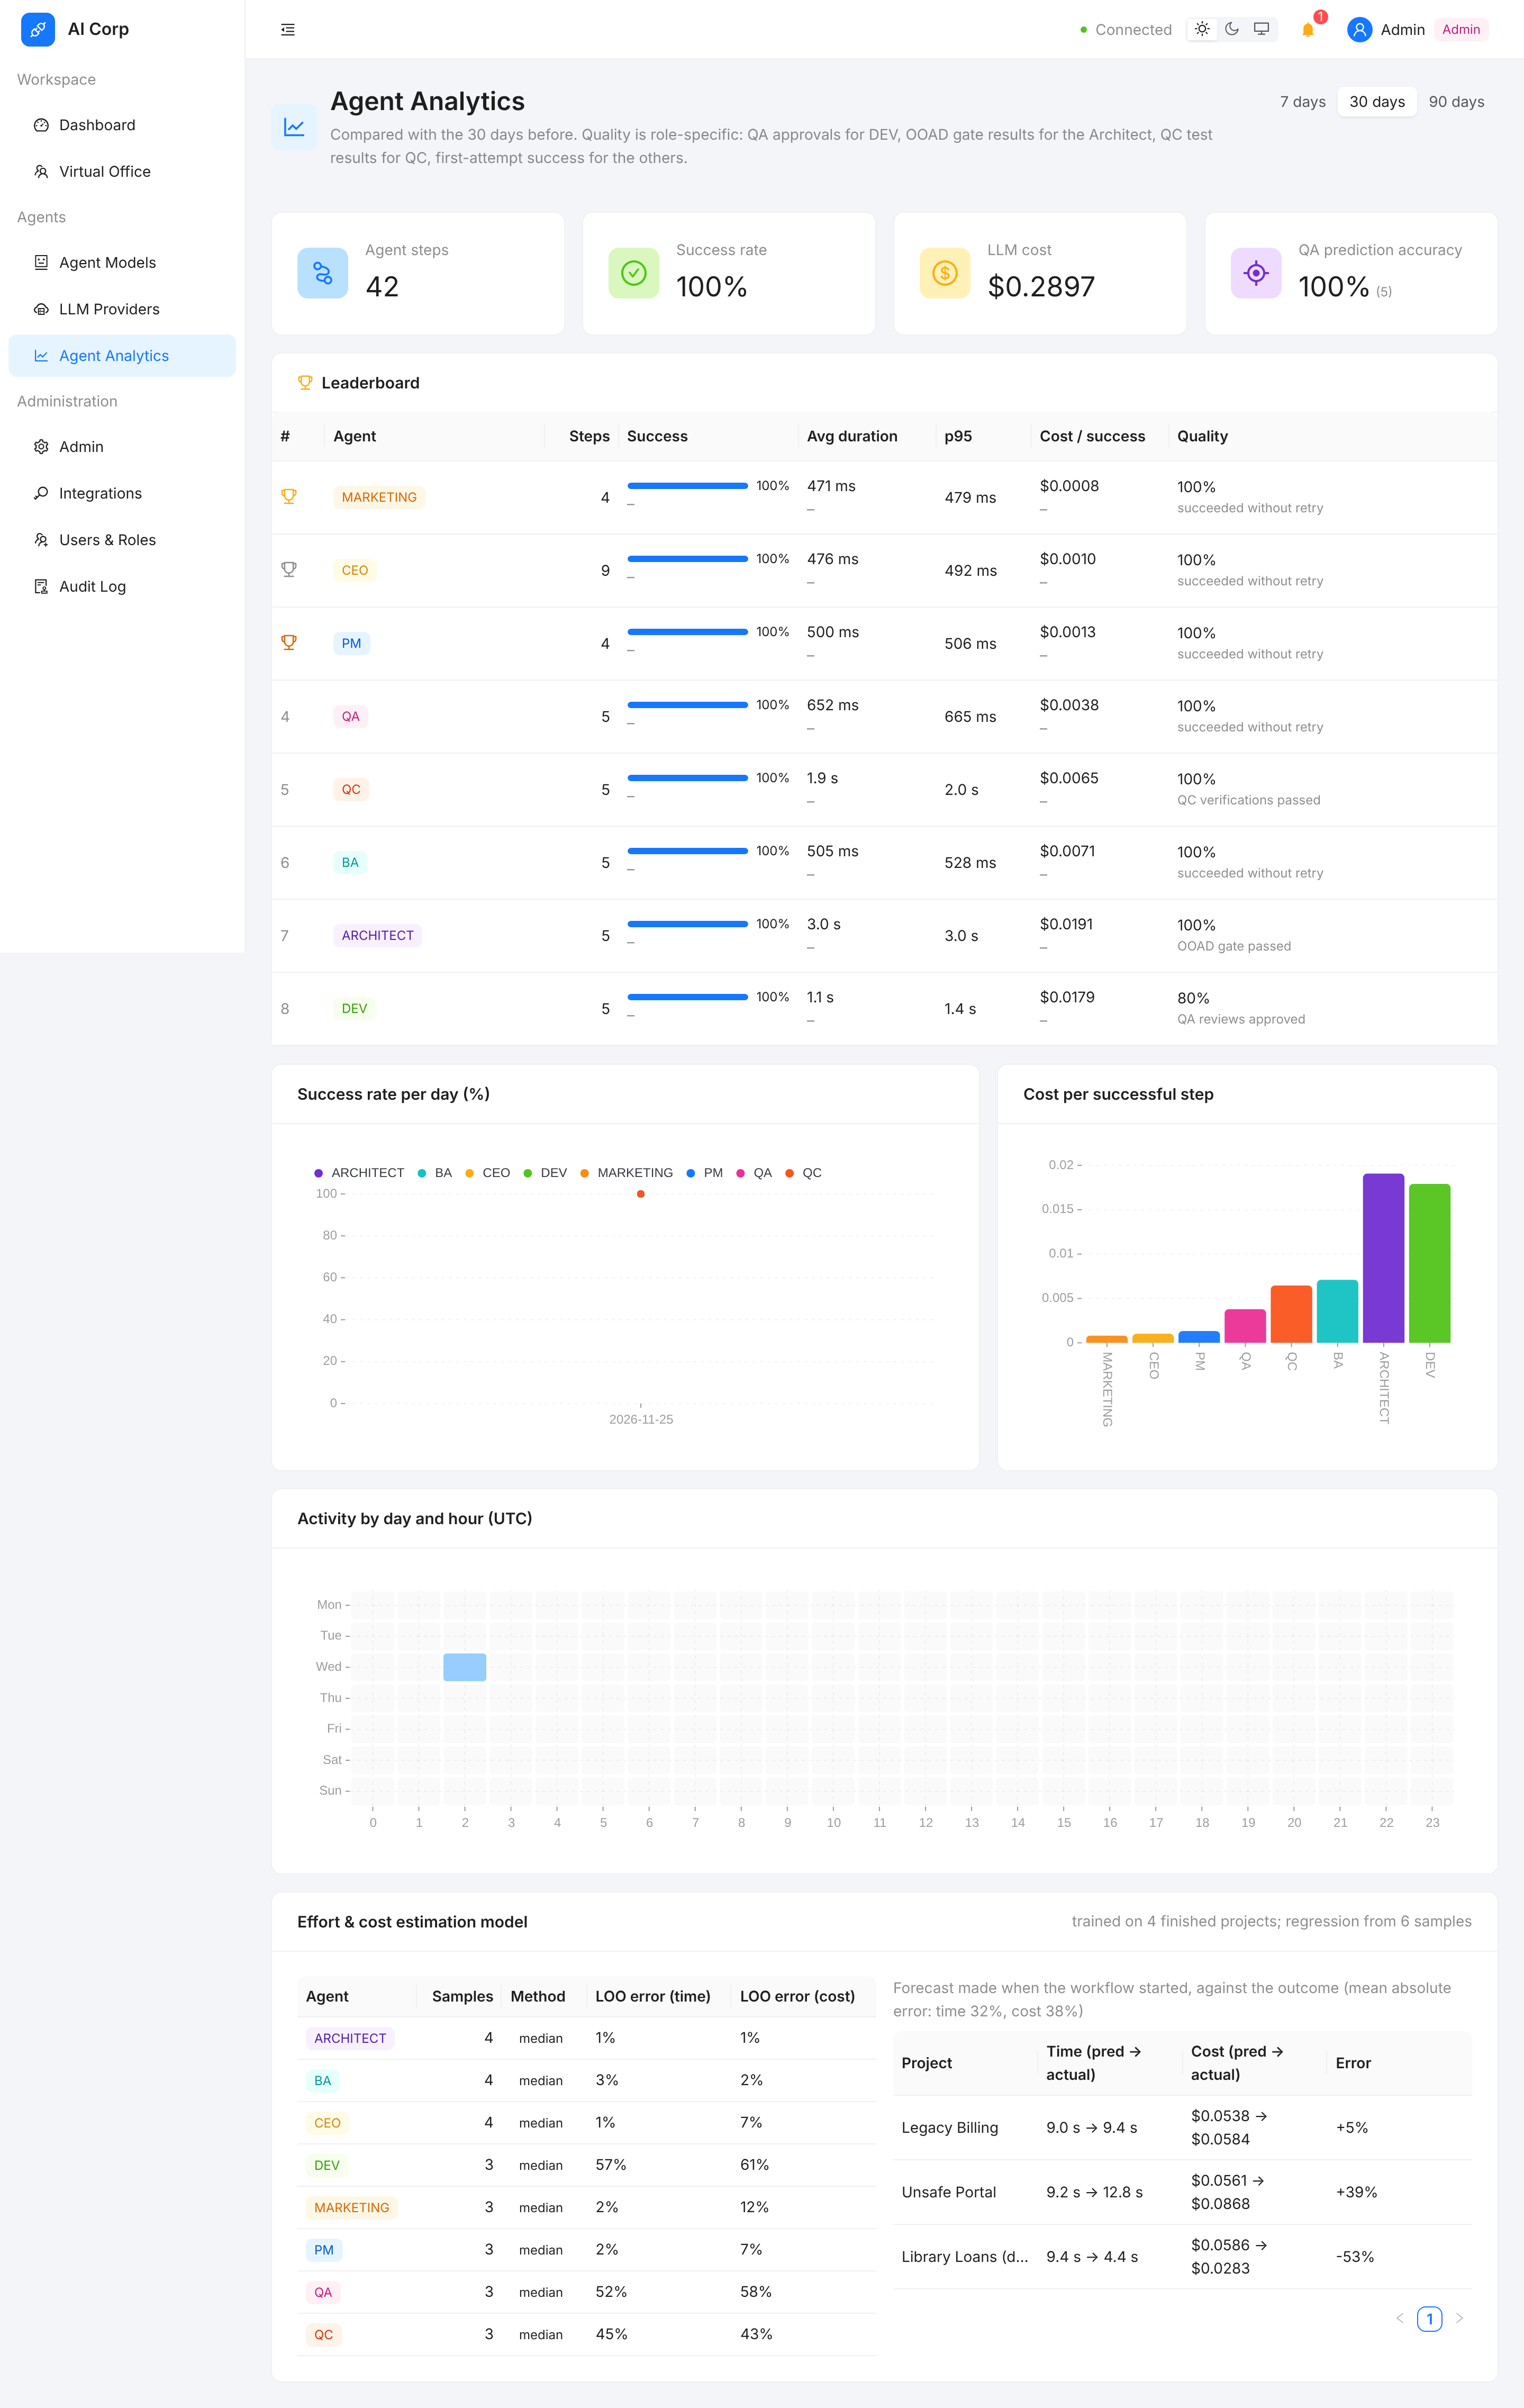
\includegraphics[height=0.75\textheight]{anh/agent-analytics.png}
\end{figure}
